\documentclass[UTF8,a4paper,zihao=-4,fontset=none]{ctexart}

\usepackage[
  top=35.0mm,
  bottom=26.0mm,
  left=30.0mm,
  right=26.0mm,
  headheight=26pt,
  headsep=2.2mm,
  footskip=6.0mm
]{geometry}
\usepackage{graphicx}
\usepackage{array}
\usepackage{setspace}
\usepackage{calc}
\usepackage{ifthen}
\usepackage{fontspec}
\usepackage{xeCJK}
\usepackage{titlesec}
\usepackage{caption}
\usepackage{fancyhdr}
\usepackage{amsmath}
\usepackage{chngcntr}
\usepackage{booktabs}
\usepackage{xcolor}
\usepackage{tocloft}
\usepackage{enumitem}
\usepackage{indentfirst}
\usepackage{url}
\usepackage{float}
\usepackage{amssymb}
\usepackage{amsmath}

\pagestyle{empty}
\setlength{\parindent}{0pt}
\setlength{\parskip}{0pt}

\setmainfont[
  Path=C:/Windows/Fonts/,
  UprightFont=times.ttf,
  BoldFont=timesbd.ttf,
  ItalicFont=timesi.ttf,
  BoldItalicFont=timesbi.ttf
]{Times New Roman}
\setCJKmainfont[
  Path=C:/Windows/Fonts/,
  UprightFont=simsun.ttc,
  AutoFakeBold=2.0
]{SimSun}
\setCJKfamilyfont{simsun}[
  Path=C:/Windows/Fonts/,
  UprightFont=simsun.ttc,
  AutoFakeBold=2.0
]{SimSun}
\setCJKfamilyfont{stxihei}[
  Path=C:/Windows/Fonts/,
  AutoFakeBold=2.2
]{STXIHEI.TTF}
\setCJKfamilyfont{stxinwei}[
  Path=C:/Windows/Fonts/,
  AutoFakeBold=2.0
]{STXINWEI.TTF}
\setCJKfamilyfont{simhei}[
  Path=C:/Windows/Fonts/,
  AutoFakeBold=2.0
]{simhei.ttf}

\newfontfamily\TimesNewRoman[
  Path=C:/Windows/Fonts/,
  UprightFont=times.ttf,
  BoldFont=timesbd.ttf,
  ItalicFont=timesi.ttf,
  BoldItalicFont=timesbi.ttf
]{Times New Roman}
\newfontfamily\Tahoma[
  Path=C:/Windows/Fonts/,
  UprightFont=tahoma.ttf,
  BoldFont=tahomabd.ttf
]{Tahoma}

% ===== 正文模板样式 =====
\newcommand{\bodyfont}{\CJKfamily{simsun}\zihao{-4}\fontsize{12pt}{22pt}\selectfont}
\newcommand{\examplefont}{\CJKfamily{simsun}\zihao{5}\fontsize{10.5pt}{22pt}\selectfont}
\newcolumntype{L}[1]{>{\raggedright\arraybackslash}p{#1}}
\setlist[enumerate]{itemsep=0pt,parsep=0pt,topsep=0pt,partopsep=0pt}

\renewcommand{\thesection}{第\arabic{section}章}
\renewcommand{\thesubsection}{\arabic{section}.\arabic{subsection}}
\renewcommand{\thesubsubsection}{\arabic{section}.\arabic{subsection}.\arabic{subsubsection}}

\titleformat{\section}
  {\centering\CJKfamily{simhei}\bfseries\zihao{3}\fontsize{16pt}{24pt}\selectfont}
  {\thesection}{1em}{}
\titlespacing*{\section}{0pt}{12pt}{24pt}

\titleformat{\subsection}
  {\CJKfamily{simhei}\bfseries\zihao{4}\fontsize{14pt}{21pt}\selectfont}
  {\thesubsection}{1em}{}
\titlespacing*{\subsection}{0pt}{10.5pt}{0pt}

\titleformat{\subsubsection}
  {\CJKfamily{simhei}\bfseries\zihao{-4}\fontsize{12pt}{18pt}\selectfont}
  {\thesubsubsection}{1em}{}
\titlespacing*{\subsubsection}{0pt}{9pt}{0pt}

\counterwithin{figure}{section}
\counterwithin{table}{section}
\numberwithin{equation}{section}
\renewcommand{\thefigure}{\arabic{section}-\arabic{figure}}
\renewcommand{\thetable}{\arabic{section}-\arabic{table}}
\renewcommand{\theequation}{\arabic{section}-\arabic{equation}}
\renewcommand{\figurename}{图}
\renewcommand{\tablename}{表}
\captionsetup{
  font={small,stretch=1.25},
  labelfont=normalfont,
  labelsep=space,
  justification=centering,
  singlelinecheck=false,
  skip=3pt
}
\captionsetup[figure]{position=bottom}
\captionsetup[table]{position=top}
\raggedbottom
\setlength{\textfloatsep}{10pt plus 2pt minus 2pt}
\setlength{\floatsep}{8pt plus 2pt minus 2pt}
\setlength{\intextsep}{10pt plus 2pt minus 2pt}
\setlength{\abovecaptionskip}{3pt}
\setlength{\belowcaptionskip}{0pt}
\setcounter{topnumber}{5}
\setcounter{bottomnumber}{5}
\setcounter{totalnumber}{10}
\renewcommand{\topfraction}{0.95}
\renewcommand{\bottomfraction}{0.85}
\renewcommand{\textfraction}{0.05}
\renewcommand{\floatpagefraction}{0.90}
\makeatletter
\setlength{\@fptop}{0pt}
\setlength{\@fpsep}{8pt plus 2pt minus 2pt}
\setlength{\@fpbot}{0pt plus 1fil}
\makeatother
\AtBeginEnvironment{figure}{\centering\CJKfamily{simsun}\zihao{5}}
\AtEndEnvironment{figure}{\bodyfont}
\AtBeginEnvironment{table}{\centering\CJKfamily{simsun}\zihao{5}}
\AtEndEnvironment{table}{\bodyfont}

\newcommand{\tocentryfont}{\CJKfamily{simsun}\TimesNewRoman\fontsize{12pt}{15pt}\selectfont}
\renewcommand{\contentsname}{目\quad 录}
\renewcommand{\cfttoctitlefont}{\hfill\CJKfamily{simhei}\bfseries\fontsize{16pt}{22pt}\selectfont}
\renewcommand{\cftaftertoctitle}{\hfill\par}
\setlength{\cftbeforetoctitleskip}{0pt}
\setlength{\cftaftertoctitleskip}{18pt}
\renewcommand{\cftsecfont}{\tocentryfont}
\renewcommand{\cftsubsecfont}{\tocentryfont}
\renewcommand{\cftsubsubsecfont}{\tocentryfont}
\renewcommand{\cftsecpagefont}{\tocentryfont}
\renewcommand{\cftsubsecpagefont}{\tocentryfont}
\renewcommand{\cftsubsubsecpagefont}{\tocentryfont}
\renewcommand{\cftsecleader}{\cftdotfill{\cftdotsep}}
\setcounter{tocdepth}{3}
\setlength{\cftsecindent}{0pt}
\setlength{\cftsubsecindent}{2em}
\setlength{\cftsubsubsecindent}{4em}
\setlength{\cftsecnumwidth}{4.8em}
\setlength{\cftsubsecnumwidth}{3.0em}
\setlength{\cftsubsubsecnumwidth}{4.2em}
\setlength{\cftbeforesecskip}{0pt}
\setlength{\cftbeforesubsecskip}{0pt}
\setlength{\cftbeforesubsubsecskip}{0pt}
\makeatletter
\newcommand{\maketemplatecontents}{%
  \clearpage
  \pagestyle{empty}
  \thispagestyle{empty}
  \begingroup
    \tocentryfont
    \setlength{\parindent}{0pt}
    {\centering\CJKfamily{simhei}\bfseries\fontsize{16pt}{22pt}\selectfont 目\quad 录\par}
    \vspace{18pt}
    \@starttoc{toc}
  \endgroup
  \clearpage
}
\makeatother

\fancypagestyle{mainstyle}{
  \fancyhf{}
  \fancyhead[C]{\textcolor{gray}{\CJKfamily{simsun}\zihao{4}人工智能基础项目报告}}
  \fancyfoot[C]{\CJKfamily{simsun}\zihao{5}\thepage}
  \renewcommand{\headrulewidth}{0.4pt}
  \renewcommand{\headrule}{\textcolor{gray}{\hrule width\headwidth height\headrulewidth \vskip-\headrulewidth}}
  \renewcommand{\footrulewidth}{0pt}
}
\newcommand{\startmainmatter}{%
  \clearpage
  \pagenumbering{arabic}
  \pagestyle{mainstyle}
  \bodyfont
  \setlength{\abovedisplayskip}{6pt plus 2pt minus 2pt}
  \setlength{\belowdisplayskip}{6pt plus 2pt minus 2pt}
  \setlength{\abovedisplayshortskip}{3pt plus 1pt minus 1pt}
  \setlength{\belowdisplayshortskip}{6pt plus 2pt minus 2pt}
  \setlength{\parindent}{2em}
  \setlength{\parskip}{0pt}
}

% ===== 封面可编辑信息 =====
\newcommand{\ChineseTitle}{基于 PyTorch 的小型 GPT 模型构建与训练}
\newcommand{\EnglishTitle}{Building and Training a Small GPT Model with PyTorch}
\newcommand{\College}{自动化学院}
\newcommand{\Major}{自动化}
\newcommand{\StudentName}{姜尹雯}
\newcommand{\StudentID}{1120233551}
\newcommand{\Supervisor}{周志强}
\newcommand{\FinishDate}{2026 年 6 月 7 日}

\newcommand{\coverlabel}[1]{{\CJKfamily{simsun}\zihao{3}#1}}
\newcommand{\covervalue}[1]{%
  \makebox[76.6mm][c]{\CJKfamily{simsun}\zihao{3}#1}%
}
\newcommand{\coverfield}[1]{%
  \makebox[76.6mm][c]{%
    \ooalign{%
      \hfil\CJKfamily{simsun}\zihao{3}#1\hfil\cr
      \raisebox{-0.42ex}{\rule{76.6mm}{0.4pt}}\cr
    }%
  }%
}
\newcommand{\coverinforow}[2]{%
  \makebox[36.4mm][r]{\coverlabel{#1}}%
  \coverfield{#2}\\[8.2mm]%
}

\newcommand{\makecover}{%
  \begin{titlepage}
    \thispagestyle{empty}
    \centering

    \vspace*{1.2mm}
    
\includegraphics[width=4.28859in,height=0.84927in]{pic/封面学校名称.png}

    \vspace{6.2mm}
    {\CJKfamily{simsun}\bfseries\fontsize{36pt}{40pt}\selectfont 人工智能基础项目报告\par}

    \vspace{19.0mm}
    {\CJKfamily{stxihei}\bfseries\fontsize{22pt}{27.5pt}\selectfont
      \parbox[c]{\textwidth}{\centering\ChineseTitle}\par}

    \vspace{6.0mm}
    {\TimesNewRoman\bfseries\fontsize{16pt}{20pt}\selectfont
      \parbox[c]{\textwidth}{\centering\EnglishTitle}\par}

    \vspace{25.0mm}
    \begin{minipage}{113.0mm}
      \coverinforow{学\quad\quad 院：}{自动化学院}
      \coverinforow{专\quad\quad 业：}{自动化}
      \coverinforow{学生姓名：}{姜尹雯}
      \coverinforow{学\quad\quad 号：}{1120233551}
      \coverinforow{指导教师：}{周志强}
    \end{minipage}

    \vfill
    {\CJKfamily{simsun}\zihao{3}\FinishDate\par}
    \vspace{11.5mm}
  \end{titlepage}
}

\begin{document}

\makecover
\maketemplatecontents
\startmainmatter

\section{绪论}

\subsection{项目背景与意义}

近年来，以 GPT 为代表的大语言模型在自然语言处理、智能问答、文本生成、代码生成等领
域得到了广泛应用。大语言模型通常基于 Transformer 结构，通过大规模文本数据训练，使
模型能够学习语言中的上下文关系和文本生成规律。与传统自然语言处理方法相比，大语言模
具有更强的通用性和迁移能力，已经成为当前人工智能领域的重要研究方向之一。

本项目以“从零构建大模型”为主题，重点并不是训练一个真正具有大规模参数量和复杂能力的
商用模型，而是在低算力平台上实现一个小参数量 GPT 类语言模型。通过完成模型搭建、文本
数据处理、预训练、微调和推理展示等过程，可以更加直观地理解大语言模型的基本结构和工
作原理，从实践角度加深对 Transformer、注意力机制、语言建模以及微调方法的认识。

\subsection{项目任务与技术路线}

根据课程作业要求，本项目需要围绕“从零构建大模型”的完整流程展开。首先，需要
梳理大语言模型构建过程中涉及的重要知识点，包括 GPT 类模型的基本架构、模型参数配
置、文本数据准备、分词方法、词嵌入、位置编码、预训练目标以及微调方法等内容。其次
，需要基于 PyTorch 搭建一个小参数量 GPT 类语言模型，使其能够在普通单机或较低算力平
台上完成训练和推理，并体现大语言模型中的核心机制。然后，需要准备小规模文本语料，完成
文本编码、训练样本构造和预训练程序设计，使模型能够通过预测下一个 token 的方式学习基
本语言规律。在此基础上，还需要构建监督微调数据，选择合适的微调任务和训练策略，使预训
练后的模型能够适应特定任务。最后，需要对实验结果进行展示和分析，总结项目完成情况、遇
到的问题以及学习收获。

本项目的整体技术路线可以概括为以下几个步骤：
\begin{enumerate}
  \item 数据准备与分词编码：选取 Hugging Face 平台上的 TinyStories 数据集作为预训练语料，对文本进行清洗和拼接，并采用基于正则表达式的分词器将文本转换为 token id 序列；
  \item 训练样本构造：利用滑动窗口方法将 token 序列切分为固定长度的输入序列，并将其右移一位作为预测目标，构成 next-token prediction 训练样本；
  \item 小型 GPT 模型搭建：基于 PyTorch 构建小参数量 GPT 类模型，主要包括词嵌入、位置嵌入、因果多头自注意力、前馈网络、残差连接和层归一化等模块；
  \item 预训练与生成测试：使用 TinyStories 样本对模型进行预训练，通过交叉熵损失优化下一个 token 的预测结果，并在训练后根据给定 prompt 进行自回归文本生成；
  \item 微调与结果分析：在预训练模型基础上构建简单监督任务进行微调，并结合 loss 曲线、perplexity、生成样例和微调结果，对模型效果进行分析总结。
\end{enumerate}

\begin{figure}[!htbp]
  \centering
  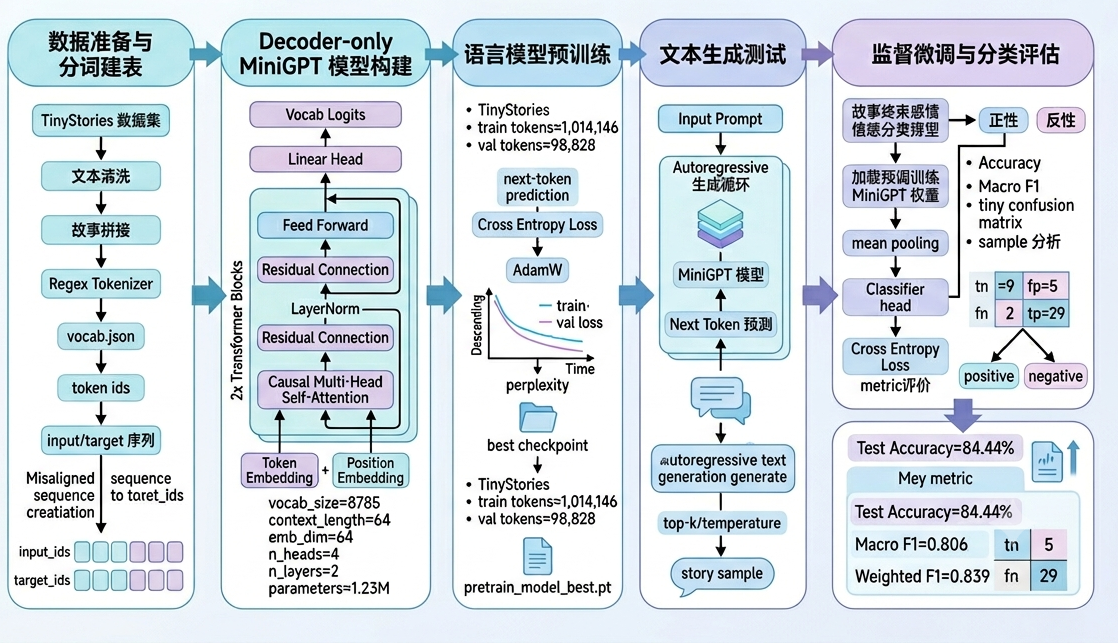
\includegraphics[width=0.96\textwidth,height=7.2cm,keepaspectratio]{pic/技术路线图.png}
  \caption{MiniGPT 项目技术路线图}
  \label{fig:technical_route}
\end{figure}

\section{大语言模型相关理论基础与关键知识点}

\subsection{从零构建语言模型的基本流程}

从零构建 GPT 类语言模型，通常不是单独完成某一个模型文件，而是一个从数据到训练、再到任务适配的完整流程。首先需要收集和整理训练语料，对原始文本进行必要清洗；随后通过分词器将文本转换为 token 序列，并建立词表和 token id 映射；接着，模型将离散 token id 转换为向量表示，送入 Decoder-only Transformer 架构；在预训练阶段，模型通过预测下一个 token 学习通用语言模式；在微调阶段，模型再根据具体任务形式和带标签数据进行适配。
上述流程对应了本报告后续章节的组织方式：第三章关注模型结
构如何实现，第四章关注预训练数据与训练过程，第五章关注
下游任务微调。本章则主要梳理这些环节背后的通用知识点，为
后文实验提供理论基础。
语言模型构建的基本流程如图~\ref{fig:LLM_building_procedure}所示。

\begin{figure}[!htbp]
  \centering
  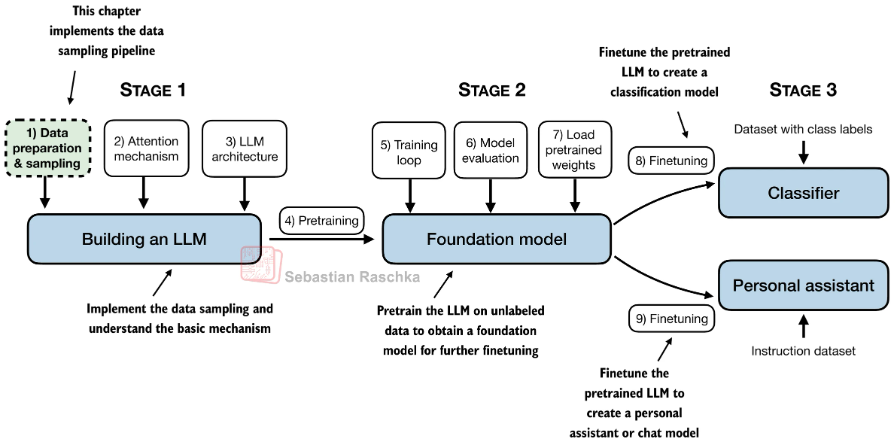
\includegraphics[width=0.85\textwidth]{pic/procedure.png}
  \caption{LLM构建基本流程图}
  \label{fig:LLM_building_procedure}
\end{figure}

\subsection{训练数据准备与文本表示}

训练数据准备的基本流程如图~\ref{fig:data_preparation} 所示。整体上，原始语料需要依次经过清洗与划分、分词编码、样本构造和批量加载，才能成为 GPT 类模型可以接收的输入。

\begin{figure}[!htbp]
  \centering
  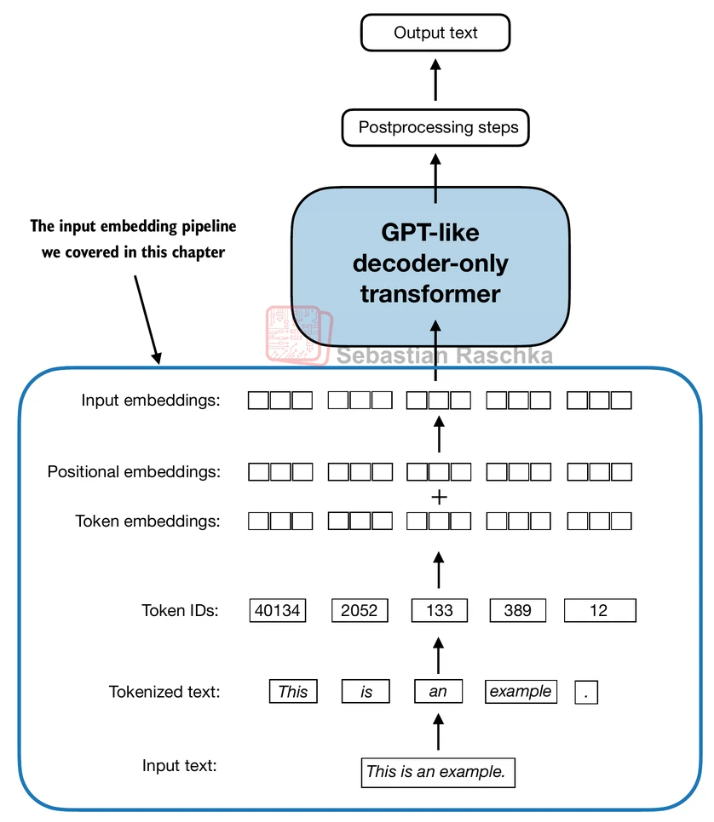
\includegraphics[width=0.47\textwidth]{pic/文本处理2.png}
  \caption{训练数据准备与文本表示流程图}
  \label{fig:data_preparation}
\end{figure}

\textbf{训练语料。} 数据准备并不只是“找到一段文本”，而是从零构建语言模型的基础环节。语言模型通过大量文本学习词语搭配、句式结构和上下文规律，因此语料的规模、质量、领域、风格和多样性都会影响模型能力。单一文本可以用于验证训练流程，但泛化能力有限；多来源、多文档语料能够提供更丰富的语言模式，有助于模型学习更稳定的统计规律。数据准备阶段的选择还会进一步影响后续分词、样本构造和预训练效果。

\textbf{文本清洗与数据划分。} 原始文本通常存在格式不统一、异常字符、空行过多或重复内容等问题，训练前需要进行适当清洗，例如统一换行格式、去除无效字符、压缩多余空白以及处理重复片段。为了判断模型是否真正学习到一般规律，而不是只记住训练文本，语料通常需要划分为训练集和验证集。如果训练集与验证集混淆，可能造成数据泄漏，使验证结果偏乐观。对于由多个文档组成的语料，还需要保留文档边界信息，避免模型把两个无关文本误认为连续上下文。

\textbf{分词、词表与特殊标记。} 原始文本不能直接输入神经网络，需要先通过分词器（tokenizer）切分为 token，再由词表映射为整数形式的 token id。token id 是模型在嵌入层之前接收的离散输入，但它本身只是整数编号，并不直接表示语义关系。图~\ref{fig:tokenization_process} 展示了文本从原始字符串转换为 token id 的基本过程。

\begin{figure}[!htbp]
  \centering
  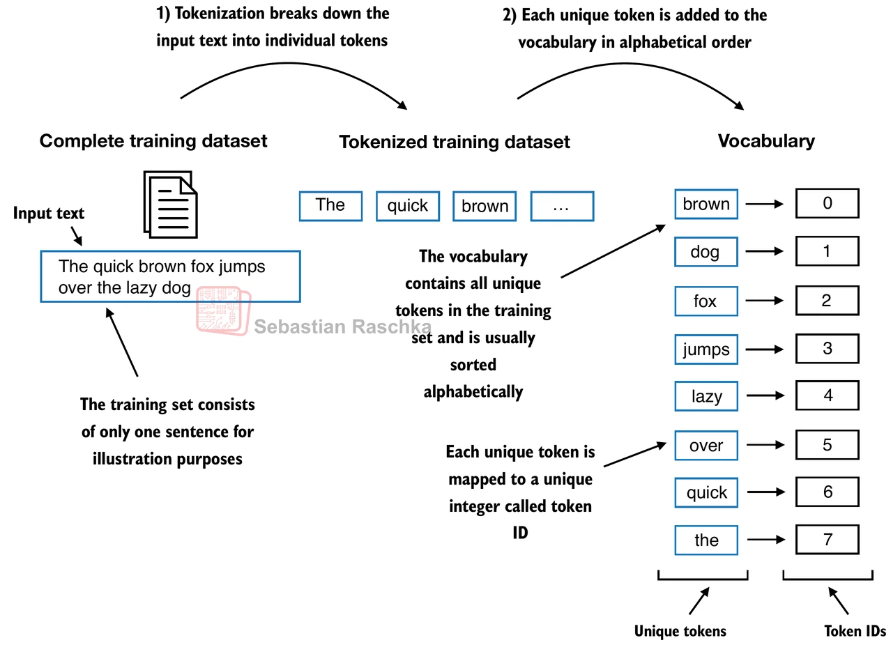
\includegraphics[width=0.85\textwidth]{pic/分词.png}
  \caption{文本输入转换流程图}
  \label{fig:tokenization_process}
\end{figure}

分词粒度会同时影响词表大小和序列长度：粒度越细，词表通常越小，但序列更长；粒度越粗，序列可能更短，但词表更大，也更容易遇到未登录词问题。实际语料中还需要使用特殊 token 表示额外信息，例如文本结束、未知词或填充（padding）位置等。在多文档拼接场景中，文本结束标记可以提示模型一个文本片段已经结束；在批量训练或分类池化时，填充位置通常不应参与有效语义建模。

\begin{table}[!htbp]
  \centering
  \caption{常见分词策略对比}
  \label{tab:tokenizer_strategy_compare}
  \renewcommand{\arraystretch}{1.2}
  \small
  \begin{tabular}{L{2.5cm}L{3.7cm}L{3.4cm}L{3.4cm}}
    \toprule
    分词方式 & 基本思想 & 优点 & 局限 \\
    \midrule
    字符级分词 & 以单个字符作为基本 token & 实现简单，词表很小 & 序列较长，生成可读性较差 \\
    词级或规则分词 & 按单词、数字、标点等规则切分 & 能保留较完整单词，含义直观 & 对未登录词和复杂词形泛化不足 \\
    BPE 子词分词 & 将常见字符组合逐步合并为子词 & 兼顾词表规模和泛化能力 & 词表和实现相对复杂，小模型开销可能较大 \\
    \bottomrule
  \end{tabular}
\end{table}

表~\ref{tab:tokenizer_strategy_compare} 对几类常见分词策略进行了概括。真实大语言模型常采用 BPE 或类似子词方法，以兼顾开放词表能力和输入效率；在小规模实验中，也可以根据语料规模、模型参数量和训练条件选择更简单的分词方案。具体到本文实验所采用的分词器，将在第四章结合预训练语料和模型规模进行说明。

\textbf{训练样本构造。} 分词和编码后，长文本会变成一条 token id 序列。语言模型通常不会把任意长度的整篇文本一次性送入模型，而是按照固定上下文长度切分为多个训练样本。常见方法是使用滑动窗口从长序列中抽取片段：每个样本的输入是一段连续 token 序列，目标序列则是输入序列整体右移一位，使模型在每个位置学习预测下一个 token。若上下文长度为 $L$，则第 $i$ 个窗口可表示为：
\begin{equation}
\mathbf{x}=(x_i,x_{i+1},\cdots,x_{i+L-1}),\quad
\mathbf{y}=(x_{i+1},x_{i+2},\cdots,x_{i+L}) .
\label{eq:sliding_window_sample}
\end{equation}
其中，$\mathbf{x}$ 为模型输入，$\mathbf{y}$ 为预测目标。窗口步长（stride）决定相邻样本之间的重叠程度：步长较小可以产生更多样本，但相邻样本高度重叠，训练开销更大，也可能增加过拟合风险；步长接近上下文长度时样本重叠较少，训练更高效，但样本数量相对减少。图~\ref{fig:sliding_window} 给出了滑动窗口样本构造示意。

\begin{figure}[!htbp]
  \centering
  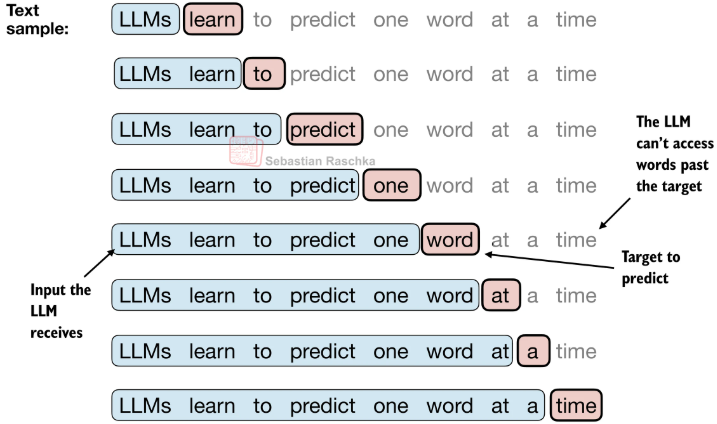
\includegraphics[width=0.65\textwidth]{pic/滑动窗口.png}
  \caption{滑动窗口样本构造示意图}
  \label{fig:sliding_window}
\end{figure}

\subsection{GPT 类模型架构与关键配置}

\subsubsection{Decoder-only Transformer 架构。} 

Transformer 的原始结构包含编码器和解码器两部分，而 GPT 类
模型主要采用解码器部分，形成 Decoder-only Transformer 架
构。该架构适合从左到右的自回归文本生成任务：模型在当前位置
进行预测时，只能利用已经出现的历史上下文。与双向理解类模型
不同，GPT 不能同时查看当前位置左右两侧的信息，因果遮罩正是
为了保证这种单向建模约
束。图~\ref{fig:llm_overall_structure} 给出了 GPT 类语言
模型从文本输入到预测分数（logits）输出的一般流程。

\begin{figure}[!htbp]
  \centering
  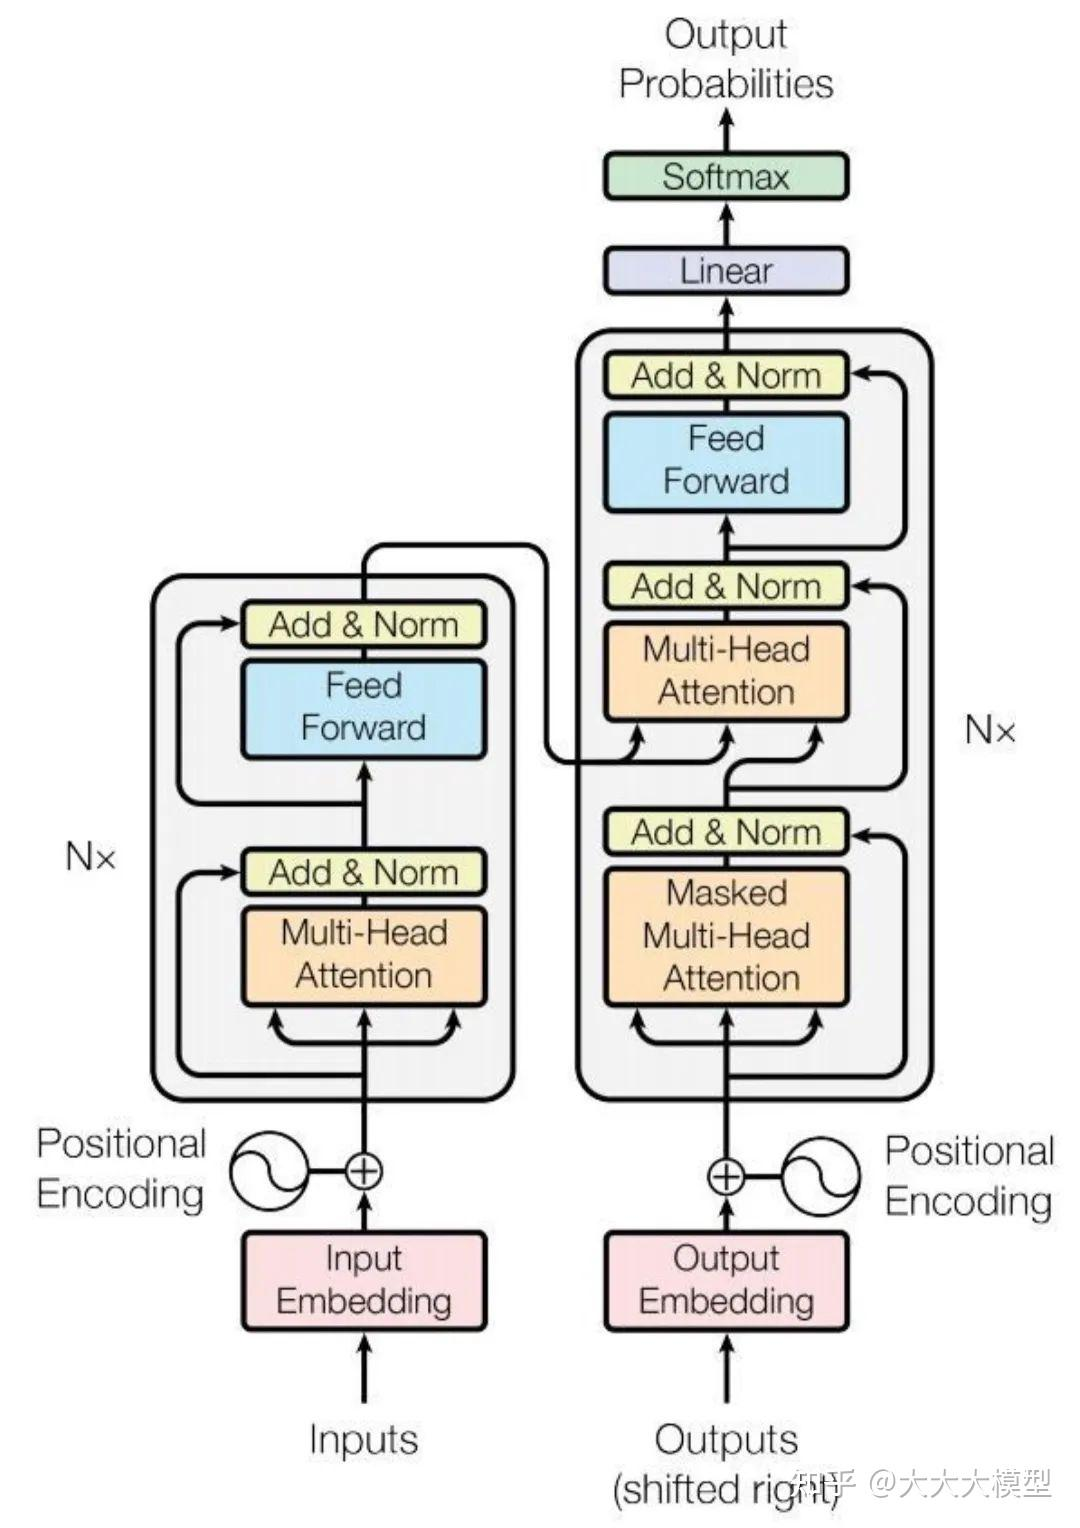
\includegraphics[width=0.92\textwidth,height=5.8cm,keepaspectratio]{pic/structure_of_llm.jpg}
  \caption{GPT 类语言模型基本流程图}
  \label{fig:llm_overall_structure}
\end{figure}

\subsubsection{模型内部模块}

\textbf{输入表示与嵌入层。} 经过分词和编码后，文本已经被表示为 token id 序列，但 token id 本身只是词表中的整数编号，编号大小并不表示语义距离。因此，GPT 类模型需要通过词嵌入（token embedding）将离散编号映射为连续向量。设词表大小为 $V$，嵌入维度为 $d$，词嵌入矩阵可表示为 $\mathbf{E}_{\mathrm{tok}}\in\mathbb{R}^{V\times d}$。对于序列中第 $t$ 个 token id $x_t$，词嵌入操作可以看作从矩阵中查找对应行向量，即 $\mathbf{e}_t=\mathbf{E}_{\mathrm{tok}}[x_t]$。在训练过程中，词嵌入矩阵会随着反向传播不断更新，使模型逐渐学习不同 token 在上下文中的表示关系。

仅有词嵌入还不足以表示文本序列。由于 Transformer 本身不像循环神经网络那样天然具有顺序建模能力，模型还需要位置嵌入（position embedding）来表示 token 在序列中的位置。若最大上下文长度为 $L$，位置嵌入矩阵可表示为 $\mathbf{E}_{\mathrm{pos}}\in\mathbb{R}^{L\times d}$。因此，第 $t$ 个位置的初始输入表示为：
\begin{equation}
\mathbf{h}^{(0)}_t
=
\mathbf{E}_{\mathrm{tok}}[x_t]
+
\mathbf{E}_{\mathrm{pos}}[t] .
\label{eq:gpt_input_embedding_single}
\end{equation}
对于整个输入序列，词嵌入和位置嵌入相加后得到初始隐藏表示：
\begin{equation}
\mathbf{H}^{(0)}
=
\mathbf{E}_{\mathrm{tok}}(\mathbf{x})
+
\mathbf{E}_{\mathrm{pos}}(\mathbf{p}) .
\label{eq:gpt_input_embedding}
\end{equation}
其中，$\mathbf{x}$ 表示 token id 序列，$\mathbf{p}$ 表示位置编号序列。这样，模型既能获得“当前 token 是什么”的内容信息，也能获得“当前 token 位于哪里”的顺序信息。

\textbf{Transformer 模块堆叠。} GPT 类模型的主体并不是由许多完全不同的模块杂糅拼接而成，而是将结构相似的 Transformer 模块重复堆叠。每个 Transformer 模块通常包含两个主要子层：因果多头自注意力子层和前馈网络子层。注意力子层负责在不同 token 之间传递上下文信息，前馈网络子层负责对每个位置的隐藏表示进行非线性变换。多个模块逐层堆叠后，模型可以不断更新每个 token 的上下文表示，从而形成更抽象的语言特征。Decoder-only Transformer 模块的典型结构如图~\ref{fig:transformer_core_structure} 所示。

\begin{figure}[!htbp]
  \centering
  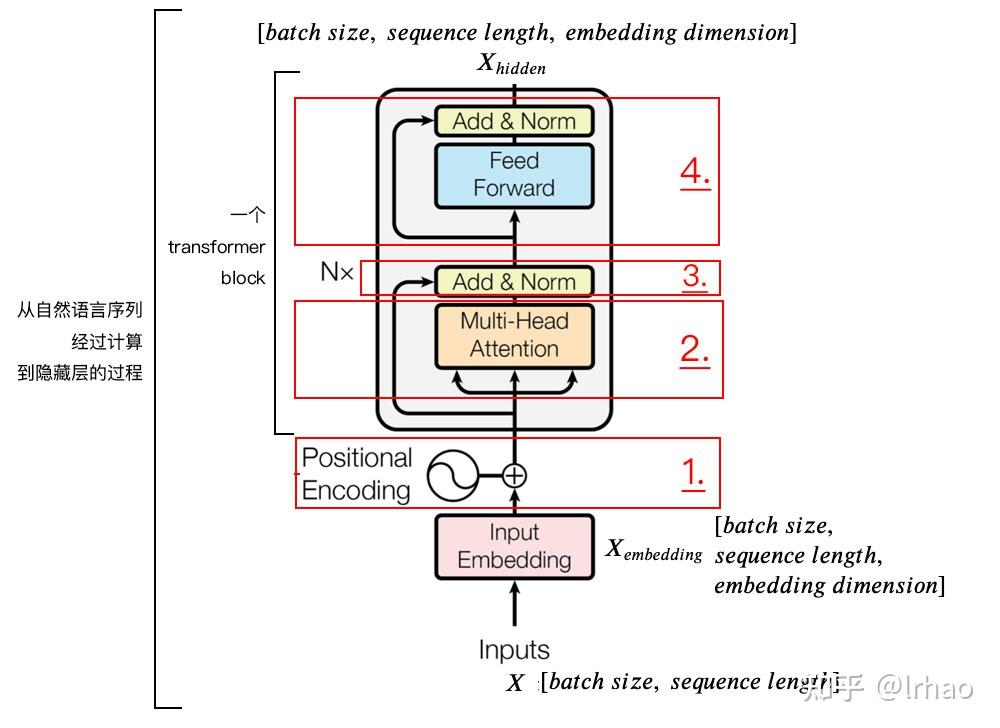
\includegraphics[width=0.90\textwidth,height=6.2cm,keepaspectratio]{pic/structure_of_transformer.jpg}
  \caption{Decoder-only Transformer 模块结构图}
  \label{fig:transformer_core_structure}
\end{figure}

\textbf{因果多头自注意力。} 自注意力机制的作用不是简单地“查看上下文”，而是为序列中每个位置重新构造一个上下文相关的表示。对于某个位置的 token，模型会计算它与其他可见位置之间的相关程度；这些相关程度经过 softmax 归一化后形成注意力权重；随后模型根据这些权重对其他位置的信息进行加权求和，得到该位置的上下文向量。这样，每个 token 的表示不再只包含自身信息，而是能够融合其上下文关系。

在带可训练参数的自注意力中，输入隐藏状态会通过线性变换得到 Query、Key 和 Value 三类向量。若某一层输入隐藏表示为 $\mathbf{H}$，则可写为 $\mathbf{Q}=\mathbf{H}\mathbf{W}_Q$、$\mathbf{K}=\mathbf{H}\mathbf{W}_K$、$\mathbf{V}=\mathbf{H}\mathbf{W}_V$。其中，Query 可以理解为当前位置发出的“查询”，表示当前位置希望查找什么上下文信息；Key 表示各位置可供匹配的特征；Value 则表示最终被汇总的信息内容。Query 与 Key 的点积用于计算注意力分数，分数越高，表示当前位置越需要关注对应位置；经过 softmax 归一化后得到注意力权重，再对 Value 加权求和，形成上下文表示。

\begin{figure}[!htbp]
  \centering
  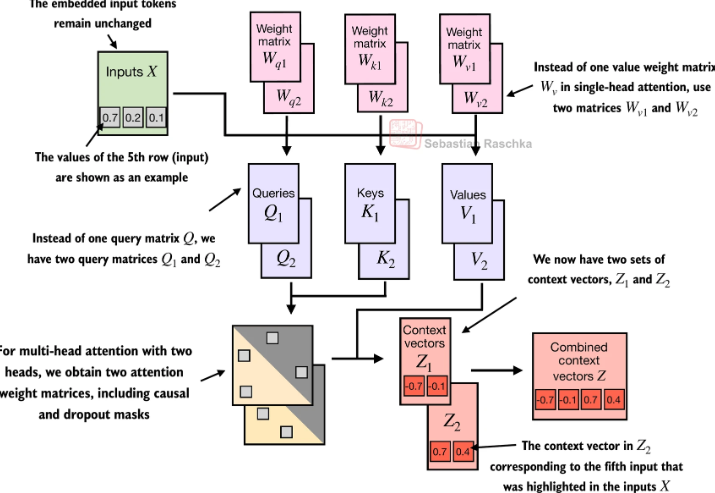
\includegraphics[width=0.60\textwidth]{pic/注意力机制示意图.png}
  \caption{ 注意力机制示意图}
  \label{fig:causal_attention}
\end{figure}

在 GPT 中，为了防止模型看到待预测 token 之后的信息，需要在注意力分数中加入因果遮罩矩阵 $\mathbf{M}$。因果注意力的核心计算形式为：
\begin{equation}
\mathrm{Attention}(\mathbf{Q},\mathbf{K},\mathbf{V})
=
\mathrm{softmax}\left(
\frac{\mathbf{Q}\mathbf{K}^{\mathrm{T}}+\mathbf{M}}{\sqrt{d_k}}
\right)\mathbf{V}.
\label{eq:causal_attention}
\end{equation}
其中，$\mathbf{Q}\mathbf{K}^{\mathrm{T}}$ 得到不同位置之间
的注意力分数；除以 $\sqrt{d_k}$ 是缩放操作，用于避免向量维度
较大时点积分数过大，使 softmax 过于集中，从而影响梯度稳定
性；$\mathbf{M}$ 表示因果遮罩矩阵，用于屏蔽未来位置；softmax
后得到注意力权重，再与 Value 相乘得到上下文表示。

在实现上，因果遮罩通常加在 softmax 之前的注意力分数上，将未来
位置的分数置为负无穷。这样经过 softmax 后，未来位置的权重
接近 $0$，而当前位置之前的可见位置仍然能够形成归一化的权重
分布。这一处理保证了 GPT 在训练和生成时都只能利用历史上下
文。在训练过程中，还可以在注意力权重或注意力输出上使用 
Dropout，以减少模型对个别位置的过度依赖，提高训练鲁棒性。

多头注意力并不是对同一注意力过程的简单重复，而是通过多组不同的线性投影，在多个表示子空间中并行建模上下文关系。若共有 $h$ 个注意力头，则第 $i$ 个头可写为 $\mathrm{head}_i=\mathrm{Attention}(\mathbf{Q}_i,\mathbf{K}_i,\mathbf{V}_i)$。多个头的输出会被拼接并再次线性映射：
\begin{equation}
\mathrm{MultiHead}(\mathbf{Q},\mathbf{K},\mathbf{V})
=
\mathrm{Concat}(\mathrm{head}_1,\mathrm{head}_2,\cdots,\mathrm{head}_h)\mathbf{W}_O .
\label{eq:multi_head_attention}
\end{equation}
不同注意力头可能关注不同类型的信息，例如局部词语搭配、句子内部结构，或距离较远但语义相关的位置。多个头的结果拼接后再经过线性投影，使模型获得更丰富的上下文表示。

\textbf{前馈网络、残差连接与层归一化。} 注意力层负责在不同 to
ken 之间传递上下文信息，而前馈网络主要作用于每个位置自身的隐藏
表示，不负责不同 token 之间的信息交换。GPT 类模型中的前馈网络
一般采用“升维—激活—降维”的结构：先将隐藏表示映射到更高维空间，
再通过非线性激活函数和线性映射回到原维度，从而增强模型表达能力
。其基本形式
可写为 $\mathrm{FFN}(\mathbf{x})=\mathbf{W}_2\,\sigma(\mathbf{W}_1\mathbf{x}+\mathbf{b}_1)+\mathbf{b}_2$，其中 $\sigma(\cdot)$ 表示非线
性激活函数。GELU 是 GPT 类模型中常用的平滑激活函数，常写
作 $\mathrm{GELU}(z)=z\Phi(z)$，其中 $\Phi(\cdot)$ 表示标准
正态分布的累积分布函数。相比简单线性变换，GELU 能够增强模型表
达非线性关系的能力。
激活函数GELU的函数曲线如图~\ref{fig:transformer_activation}所示。

\begin{figure}[!htbp]
  \centering
  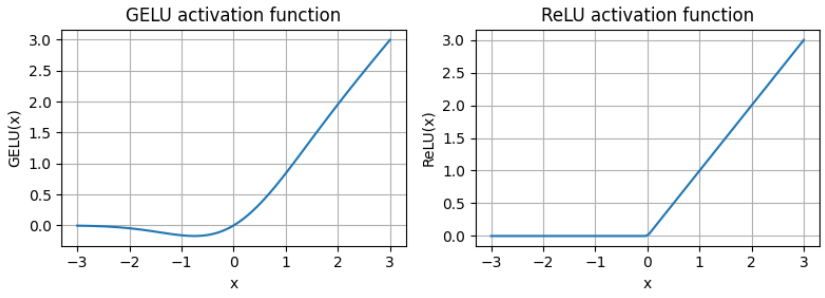
\includegraphics[width=0.60\textwidth]{pic/激活函数.png}
  \caption{激活函数}
  \label{fig:transformer_activation}
\end{figure}

残差连接使子层输入可以直接传递到子层输出，避免深层网络在多次变
换后过早丢失原始信息。同时，残差路径也为梯度反向传播提供了更直
接的通道，有助于缓解深层模型训练困难。若将某个子层
记为 $\mathcal{F}(\cdot)$，残差连接可简
写为 $\mathbf{y}=\mathbf{x}+\mathcal{F}(\mathbf{x})$。因
此，残差连接不是附加细节，而是 GPT 类模型能够稳定堆叠多层 Tra
nsformer 模块的重要条件。

\begin{figure}[!htbp]
  \centering
  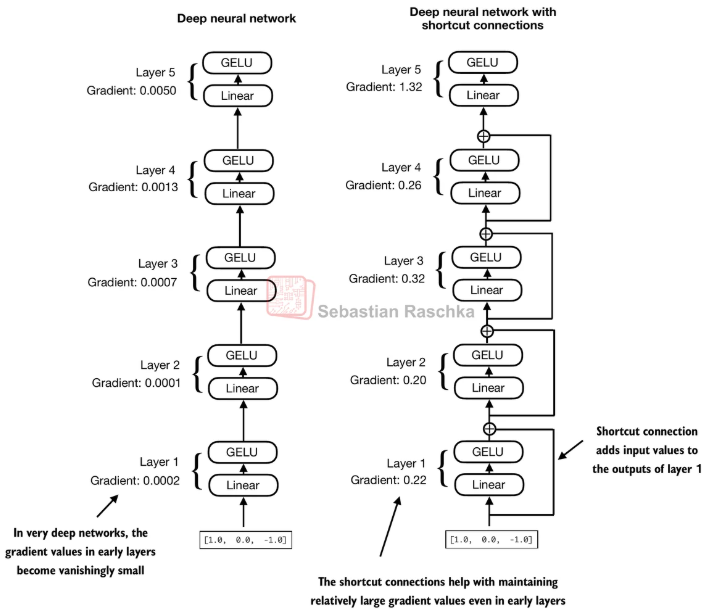
\includegraphics[width=0.60\textwidth]{pic/残差链接示意图.png}
  \caption{残差连接示意图}
  \label{fig:shortcut_connection}
\end{figure}

层归一化（LayerNorm）用于稳定每个 token 的隐藏表示，通常在特
征维度上进行归一化，使不同层之间的数值分布更稳定。对某个隐藏向
量 $\mathbf{x}$，层归一化可以写为：
\begin{equation}
\mathrm{LayerNorm}(\mathbf{x})
=
\boldsymbol{\gamma}
\odot
\frac{\mathbf{x}-\mu}{\sqrt{\sigma^2+\epsilon}}
+
\boldsymbol{\beta}.
\label{eq:layer_norm}
\end{equation}
其中，$\mu$ 和 $\sigma^2$ 分别表示该隐藏向量在特征维度上的
均值和方差，$\boldsymbol{\gamma}$ 与 $\boldsymbol{\beta}$ 是
可学习的缩放和平移参数。层归一化不改变序列长度，而是调整每个位置
的隐藏向量，并通过可学习参数保留表达能力。层归一化的简单示意
如图~\ref{fig:layer_norm}所示。

\begin{figure}[!htbp]
  \centering
  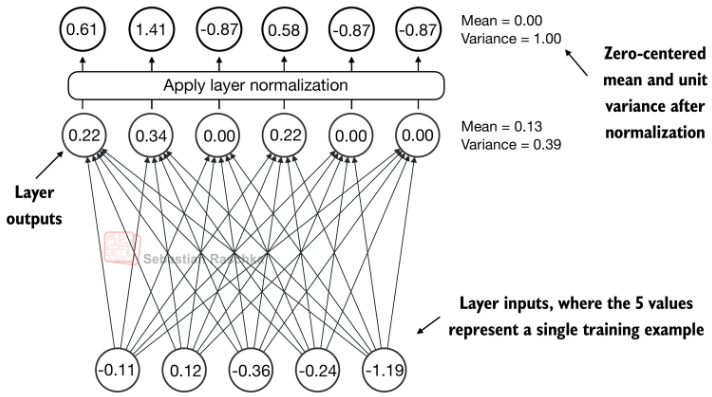
\includegraphics[width=0.60\textwidth]{pic/层归一化.png}
  \caption{层归一化示意图}
  \label{fig:layer_norm}
\end{figure}

在 Transformer 模块中，层归一化可以放在子层之前或之后。GPT 
类实现中常见的一种形式是 Pre-LayerNorm，即先对输入隐藏状态
进行层归一化，再送入注意力子层或前馈网络子层，最后与原输入进行
残差相加。若第 $l$ 层输入为 $\mathbf{H}^{(l)}$，一种 Pre-L
ayerNorm 结构可概括为：
\begin{equation}
\begin{aligned}
\widetilde{\mathbf{H}}^{(l)}
&=
\mathbf{H}^{(l)}
+
\mathrm{Attn}\!\left(\mathrm{LayerNorm}(\mathbf{H}^{(l)})\right),\\
\mathbf{H}^{(l+1)}
&=
\widetilde{\mathbf{H}}^{(l)}
+
\mathrm{FFN}\!\left(\mathrm{LayerNorm}(\widetilde{\mathbf{H}}^{(l)})\right).
\end{aligned}
\label{eq:pre_layer_norm_block}
\end{equation}
相比直接在子层输出之后归一化，Pre-LayerNorm 往往更有利于深层
模型的稳定训练。

\textbf{输出层与生成过程。} 经过多层 Transformer 模块后，序列中每个位
置都会得到一个上下文相关的隐藏表示。最终层归一化用于进一步稳定输出表示，
线性输出层则将隐藏表示映射到词表维度，得到每个候选 token 的预测分数。若
最后一层隐藏表示为 $\mathbf{H}^{(N)}$，输出层可写
为 $\mathbf{Z}=\mathbf{H}^{(N)}\mathbf{W}_{\mathrm{out}}$，其
中 $\mathbf{Z}$ 的最后一维对应词表中每个 token 的预测分数。训练阶
段，这些预测分数用于与目标 token 计算语言模型损失；生成阶段，模型
通常取最后一个位置的预测分布来选择下一个 token，并将新 token 拼接
回上下文继续生成。

\begin{figure}[!htbp]
  \centering
  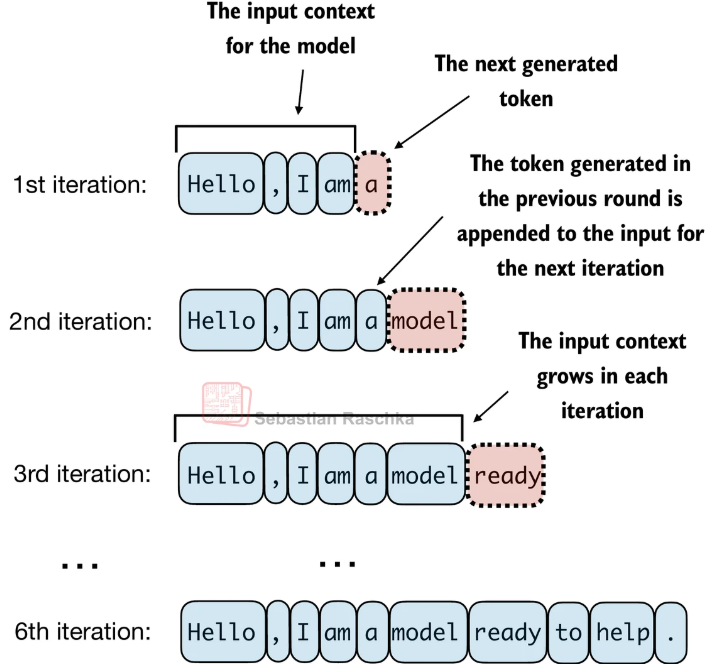
\includegraphics[width=0.50\textwidth]{pic/单词续写示例.png}
  \caption{单词续写示例}
  \label{fig:text_generation}
\end{figure}

GPT 的自回归生成过程并不是一次性输出完整文本，而是每次根据当前上下文
得到下一个 token 的概率分布。若当前上下文为 $x_{\leq t}$，最后一个
位置的预测分数为 $\mathbf{z}_t$，则下一个 token 的概率分布可表
示为 $P(x_{t+1}\mid x_{\leq t})=\mathrm{softmax}(\mathbf{z}_t)$。生
成时通常从该分布中采样或选择下一个 token。新 token 被追加到上下文后，
模型再重复前向计算，直到达到长度限制或生成终止标记。

\subsubsection{关键配置}

GPT 类模型的配置不是随意设置的，而是在模型表达能力、训练成本和硬件资源之间进行权衡。模型参数主要来自词嵌入层、注意力层、前馈网络和最终输出层。词表大小会显著影响词嵌入层和输出层参数量；注意力层中的 Query、Key、Value 投影和输出投影会带来参数开销；前馈网络由于包含升维和降维线性层，通常也占据较多参数。上下文长度决定模型最多能利用多长的历史信息，同时注意力计算开销会随序列长度增加而明显上升；嵌入维度影响 token 表示空间的容量；Transformer 层数影响模型抽象能力和训练成本；注意力头数影响模型从不同子空间捕捉关系的能力，但也需要与嵌入维度匹配。除此之外，Dropout、权重衰减等正则化方法有助于减少过拟合，批大小和学习率则会影响训练稳定性和收敛速度。具体配置需要根据数据规模、计算资源和实验目标综合确定，相关数值设置将在后文章节结合具体实验说明。

\subsection{模型预训练机制}

预训练是 GPT 类语言模型获得通用语言能力的核心阶段。与需要人工标签的监督学习不同，语言模型预训练通常直接利用无标签文本构造训练目标。对于自回归语言模型而言，文本序列本身就能提供监督信号：模型根据已有上下文预测下一个 token，并通过预测结果与真实下一个 token 之间的误差更新参数。因此，GPT 预训练可以看作一种自监督学习过程。

\subsubsection{模型评估标准}

在预训练阶段，最基本的评估指标是训练损失和验证损失。训练损失（training loss）是在训练集 batch 上计算得到的平均交叉熵损失，用于反映模型对训练语料的拟合程度；验证损失（validation loss）是在不参与参数更新的验证集上计算得到的损失，用于反映模型在未见文本上的泛化能力。二者的变化趋势可以帮助判断模型是否正常收敛。

给定 token 序列 $x_1,x_2,\cdots,x_T$，GPT 类模型通过下一个 token 预测任务进行预训练，其语言建模目标可写为：
\begin{equation}
\begin{aligned}
P(x_1,x_2,\cdots,x_T)
&=\prod_{t=1}^{T}P(x_t\mid x_{<t}),\\
\mathcal{L}_{\mathrm{LM}}
&=-\frac{1}{T-1}\sum_{t=1}^{T-1}
\log P(x_{t+1}\mid x_{\leq t}) .
\end{aligned}
\label{eq:pretraining_objective}
\end{equation}
其中，第一行表示自回归概率分解，第二行表示平均交叉熵损失。模型在每个位置输出词表维度的预测分数，经 softmax 后得到下一个 token 的概率分布，训练目标则是提高真实目标 token 的概率。

训练损失和验证损失需要结合观察。如果训练损失和验证损失都持续下降，通常说明模型正在学习较稳定的语言规律；如果训练损失下降而验证损失不再下降甚至上升，则说明模型可能逐渐记住训练语料，出现过拟合。由此可见，验证损失并不是训练过程中的附加指标，而是模型选择和判断泛化能力的重要依据。

语言模型中还常使用困惑度（perplexity）辅助评价模型效果。困惑度通常由语言模型损失指数变换得到：
\[
\mathrm{PPL}=\exp(\mathcal{L}_{\mathrm{LM}}).
\]
直观上，困惑度可以理解为模型预测下一个 token 时的平均不确定程度。困惑度越低，通常表示模型对真实下一个 token 的预测越稳定。需要注意的是，困惑度会受到分词方式和词表规模影响，因此不同 tokenizer 或不同词表设置下的数值不能简单横向比较。

\subsubsection{预训练过程}

模型预训练并不只是计算一次损失，而是一个按照 epoch 重复进行
的迭代优化过程。每个 epoch 中，模型会遍历训练集中的多个 bat
ch，通过前向传播、损失计算、反向传播和参数更新逐步调整模型
参数，并定期在验证集上评估训练效果。

\begin{figure}[!htbp]
  \centering
  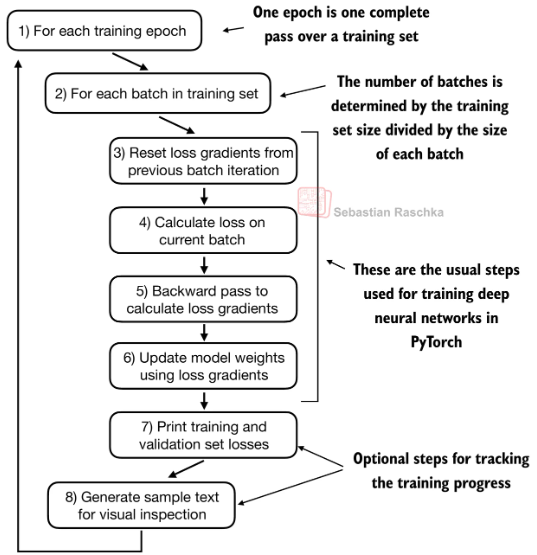
\includegraphics[width=0.50\textwidth]{pic/预训练流程.png}
  \caption{预训练流程示意}
  \label{fig:pretraining_process}
\end{figure}

\textbf{模型进入训练模式。} 在每个 epoch 开始时，模型通常会切换到训练模式，使 Dropout 等训练阶段才启用的机制正常工作。随后，数据加载器按 batch 提供输入序列和目标序列。输入序列用于送入模型，目标序列通常是输入序列整体右移一位后的 token 序列。

\textbf{前向传播。} 对于一个 batch，模型接收形状通常为 $[\mathrm{batch\_size},\mathrm{context\_length}]$ 的 token id 张量。经过词嵌入、位置嵌入和多层 Transformer 模块后，模型在每个位置输出词表维度的预测分数。若词表大小为 $V$，则输出可以表示为 $[\mathrm{batch\_size},\mathrm{context\_length},V]$。

\textbf{损失计算。} 模型输出的预测分数需要与目标 token 计算交叉熵损失。由于每个位置都要预测下一个 token，因此损失通常会在整个 batch 的所有有效位置上求平均。该损失值越小，说明模型越能给真实下一个 token 分配较高概率。

\textbf{反向传播与参数更新。} 得到损失后，程序通过反向传播计算模型参数的梯度，再由优化器根据梯度更新参数。常见做法是在每个 batch 更新前清空上一轮梯度，完成损失反向传播后执行一次优化器更新。这样，模型会随着训练不断调整词嵌入、注意力层、前馈网络和输出层等参数。

\textbf{验证集评估。} 训练过程中需要定期在验证集上计算损失。验证阶段通常关闭梯度计算，并将模型切换到评估模式，以避免 Dropout 等训练随机性影响评估结果。验证损失可以反映模型在未参与训练文本上的表现，是判断训练是否有效和是否过拟合的重要依据。

\textbf{记录与模型选择。} 每轮或每隔一定步数记录训练损失、验证损失以及困惑度，有助于后续绘制曲线并分析收敛情况。若当前验证损失优于历史结果，通常会保存当前模型作为最优模型；训练结束时也会保存最后一轮模型，便于后续比较、继续训练或进行微调。

\subsubsection{Decoding Strategies（解码策略）}

预训练完成后，可以通过文本生成直观观察模型是否学到基本语言模式。生成时，模型根据给定 prompt 预测下一个 token，再将生成的 token 拼接回上下文中，重复这一过程直到达到长度限制或生成终止标记。

最简单的解码方式是贪心解码，即每一步都选择概率最高的 token。这种方式结果较稳定，但容易生成重复或缺乏变化的文本。为了增加生成多样性，可以使用 temperature 对预测分数进行缩放：
\[
P_i=\mathrm{softmax}\left(\frac{z_i}{\tau}\right).
\]
其中，$\tau$ 为温度系数。较小的 $\tau$ 会使概率分布更尖锐，模型更倾向于选择高概率 token；较大的 $\tau$ 会使分布更平滑，生成结果更随机。此外，top-k 采样会把候选范围限制在概率最高的 $k$ 个 token 内，在保留一定随机性的同时减少明显不合理 token 被采样的可能性。

\subsubsection{Loading and Saving Model（模型加载与保存）}

由于语言模型预训练通常耗时较长，训练过程中需要保存模型权重和相关训练信息。常见保存内容包括模型参数、模型配置、词表文件、训练参数和评估指标等。保存最后一轮模型可以保留完整训练结果，保存验证损失最低的模型则便于后续选择泛化表现较好的版本。

模型加载通常用于三类场景：一是继续中断的预训练过程；二是加载预训练模型进行文本生成测试；三是在预训练模型基础上进行下游任务微调。对于后续微调而言，除了加载模型权重，还需要保证 tokenizer 和词表与预训练阶段一致，否则相同文本可能被编码为不同 token id，导致模型输入表示不匹配。因此，模型保存与加载不仅是工程实现细节，也是保证预训练、生成和微调流程连续性的关键环节。

\subsection{模型微调与任务适配}

预训练阶段主要使 GPT 类模型学习通用语言模式，但实际应用往
往具有明确的任务目标，例如文本分类、问答、摘要、指令响应等
。因此，在预训练之后，还需要通过微调使模型适应具体任务。微
调的基本思想是：在保留预训练模型已有语言表示能力的基础上
，使用带标签数据或任务格式数据继续训练模型，使模型的输出
形式和目标任务相匹配。本节主要介绍文本
分类微调和指令跟随微调。

\subsubsection{文本分类任务微调}

文本分类任务要求模型根据输入文本判断其所属类别，例如情感分
类、垃圾短信识别、主题分类等。与预训练阶段的下一个 token
预测不同，文本分类任务的输出不是一段连续文本，而是一个离
散类别。因此，分类微调需要在 GPT 主体模型之后增加任务相
关的分类结构，使预训练语言模型能够从“生成式建模”适配到“
类别判断”。

\begin{figure}[!htbp]
  \centering
  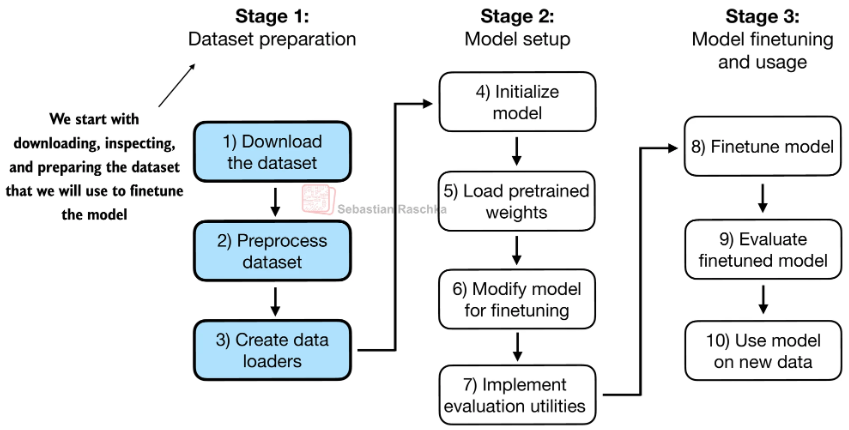
\includegraphics[width=0.60\textwidth]{pic/分类微调流程.png}
  \caption{文本分类任务微调流程}
  \label{fig:classification_finetuning}
\end{figure}

\textbf{数据集准备。} 文本分类微调首先需要构建带标签数据集。每条样本通常由两部分组成：一部分是输入文本，另一部分是人工标注或已有数据集中提供的类别标签。为了能够输入 GPT 模型，文本仍然需要使用与预训练阶段一致的分词器进行编码，转换为 token id 序列。由于不同文本长度可能不同，实际训练时通常需要进行截断或填充，使同一批次中的样本具有统一长度。对于填充位置，需要通过有效位置标记进行区分，避免其影响文本表示或损失计算。

分类数据集还需要划分为训练集、验证集和测试集。训练集用于更新模型参数，验证集用于观察微调过程和选择模型，测试集用于最终评价模型在未见样本上的表现。若类别分布不均衡，仅使用准确率可能无法全面反映模型效果，因此通常还需要结合精确率、召回率、F1 值和混淆矩阵等指标进行分析。

\textbf{模型设置。} GPT 主体模型输出的是每个 token 对应的隐藏状态，而文本分类任务需要对整段文本给出一个整体判断，因此需要将 token 级表示转换为文本级表示。常见做法包括使用最后一个有效 token 的隐藏状态、对所有有效 token 的隐藏状态进行平均池化，或采用最大池化等方式。最后一个 token 表示更接近自回归生成任务的习惯，但可能过度依赖序列末尾信息；平均池化能够综合整段文本的表示，更适合需要整体语义判断的短文本分类任务；最大池化则更强调局部显著特征。

得到文本级表示后，需要在其后接入线性分类头，将隐藏表示映射为类别预测分数。设文本级表示为 $\mathbf{h}$，分类头参数为 $\mathbf{W}_c$ 和 $\mathbf{b}_c$，则类别预测分数可以写为 $\mathbf{z}=\mathbf{h}\mathbf{W}_c+\mathbf{b}_c$。经过 softmax 后，模型得到各类别的预测概率。若真实类别为 $y$，则分类交叉熵损失可表示为：
\[
\mathcal{L}_{\mathrm{cls}}=-\log p_y .
\]
该损失鼓励模型提高真实类别对应的预测概率，从而学习输入文本与类别标签之间的对应关系。

在参数更新策略上，文本分类微调可以采用多种方式。一种做法是冻结预训练 GPT 主体，只训练新增分类头，这种方式训练成本较低，但任务适配能力有限；另一种做法是全参数微调，即 GPT 主体和分类头全部参与训练，适配能力更强，但训练开销更大，也更容易在小数据集上过拟合。实际选择时需要根据模型规模、数据量和算力条件进行权衡。

\textbf{模型微调与使用。} 文本分类微调的训练过程与一般监督学习类似。每个 batch 中，模型先对输入文本进行前向传播，得到类别预测分数；然后与真实标签计算分类损失；接着通过反向传播计算梯度，并由优化器更新分类头以及参与训练的模型参数。训练过程中需要定期在验证集上评估模型表现，防止训练集损失下降但验证集效果变差。

微调完成后，模型即可用于分类推理。对于一段新的输入文本，程序首先使用同一分词器进行编码，再送入微调后的模型，得到类别预测分数，最后选择概率最高的类别作为输出。与预训练阶段相比，分类微调后的模型不再只是生成下一个 token，而是能够面向具体监督任务输出明确类别。因此，文本分类微调常用于验证预训练模型是否能够迁移到下游任务中。

\subsubsection{指令跟随微调}

指令跟随微调是一类更接近实际大语言模型应用的微调方式。它的
目标不是让模型输出固定类别，而是让模型根据自然语言指令生成
符合要求的回答。例如，用户可以要求模型翻译句子、总结文本、
回答问题或改写内容，模型需要理解指令意图，并生成相应响应。
与文本分类微调相比，指令跟随微调仍然保持生成式输出形式，但
训练数据需要按照“指令—输入—回答”的格式组织。

\begin{figure}[!htbp]
  \centering
  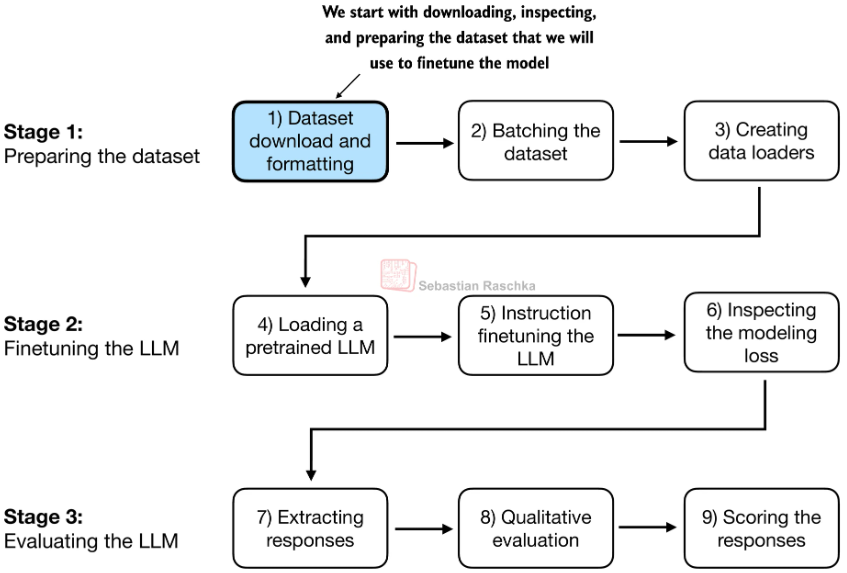
\includegraphics[width=0.60\textwidth]{pic/指令微调流程.png}
  \caption{指令跟随微调流程}  
  \label{fig:instruction_finetuning}
\end{figure}

\textbf{数据集准备。} 指令微调数据通常由三部分组成：指令、输入和回答。指令用于说明任务要求，输入提供任务所需的具体内容，回答则是期望模型生成的目标文本。例如，一条样本可以包含“请总结下面这段文字”这样的指令、待总结的原文，以及对应的参考摘要。对于不需要额外输入的任务，也可以只包含指令和回答。

为了便于训练，不同样本通常需要整理成统一模板。例如，可以
将样本拼接为“Instruction + Input + Response”的形式，
使模型在看到前面的指令和输入后，学习生成后面的回答。与普通预训练不同，指令微调更强调输入输出格式的一致性。如果模板设计混乱，模型可能难以学习到指令和回答之间的对应关系。

由于指令样本长度不一，训练时同样需要进行分词、截断、填充和批量组织。对于填充部分，应避免其参与损失计算。对于指令和输入部分，某些实现也会选择不计算损失，而只对回答部分计算损失，使模型更集中地学习如何生成目标响应。

\textbf{微调大语言模型。} 指令跟随微调本质上仍然可以使用自回归语言建模目标。模型接收由指令、输入和回答拼接而成的序列，并学习在给定前文条件下预测后续 token。不同之处在于，训练目标不再是普通文本续写，而是在特定任务说明下生成符合要求的回答。

若一条样本被组织为：
“Instruction + Input + Response”
则模型需要根据指令和输入部分生成回答部分。实际训练中，可以对不需要学习的 token 位置设置忽略标记，使损失主要作用在回答 token 上。这样做可以避免模型把大量训练能力浪费在重复输入提示格式上，而是更关注如何生成符合指令要求的输出。

指令微调的参数更新方式可以是全参数微调，也可以是参数高效微调。全参数微调会更新模型全部参数，适配能力较强，但训练成本高；参数高效方法通常只更新少量新增参数或低秩适配模块，适合大模型和有限算力环境。无论采用哪种方式，都需要保证微调阶段使用的分词器、词表和模型结构与预训练阶段保持一致，否则模型输入表示会出现不匹配。

\textbf{评估大语言模型。} 指令跟随微调的评估比文本分类更复杂。分类任务通常有明确标签，可以直接计算准确率、F1 值等指标；而指令回答往往不存在唯一标准答案，即使两个回答内容不同，也可能都满足任务要求。因此，指令微调模型的评估通常需要结合自动指标和人工判断。

对于摘要、翻译等任务，可以使用与参考答案的重合度指标进行初步评价；对于开放式问答、写作和对话任务，则更关注回答是否正确、完整、符合指令、语言是否流畅以及是否存在事实错误。实际应用中，也可以通过人工评分或更强模型辅助评价的方式比较不同模型输出质量。由于评价成本较高，指令跟随微调通常比文本分类微调更复杂，也更依赖高质量数据和合理的评估标准。

总体来看，文本分类微调更适合用来验证预训练模型的基础任务适配能力，而指令跟随微调更接近实际大语言模型助手的训练方式。前者输出形式简单、指标明确，后者任务形式灵活、应用范围更广。本文后续实验选择文本分类任务作为监督微调示例，指令跟随微调则可作为进一步扩展方向。



\section{小型 GPT 模型设计与实现}

\subsection{模型总体结构}

本项目实现的是一个小参数量 Decoder-only GPT 类语言模型，其目标是在普通单机和较低算力
条件下完成模型结构验证、预训练和推理生成实验。模型输入为 token id 序列，形状为
$[\mathrm{batch\_size},\mathrm{seq\_len}]$；模型输出为 logits，形状为
$[\mathrm{batch\_size},\mathrm{seq\_len},\mathrm{vocab\_size}]$。其中，最后一维对应
词表中每个 token 的预测分数，可用于预训练阶段的 next-token prediction 损失计算，也可
用于推理阶段选择下一个 token。

从整体结构看，\texttt{MiniGPT} 包含词嵌入、位置嵌入、嵌入 Dropout、
多层 \texttt{TransformerBlock}、最终 LayerNorm 以及无偏置线性输出层。该结构
与第二章介绍的 GPT 基本原理一致，但参数规模明显减小，更适合课程实验中对大语言模型核
心机制进行复现和验证。模型总体结构如图~\ref{fig:minigpt_structure} 所示。

\begin{figure}[!htbp]
  \centering
  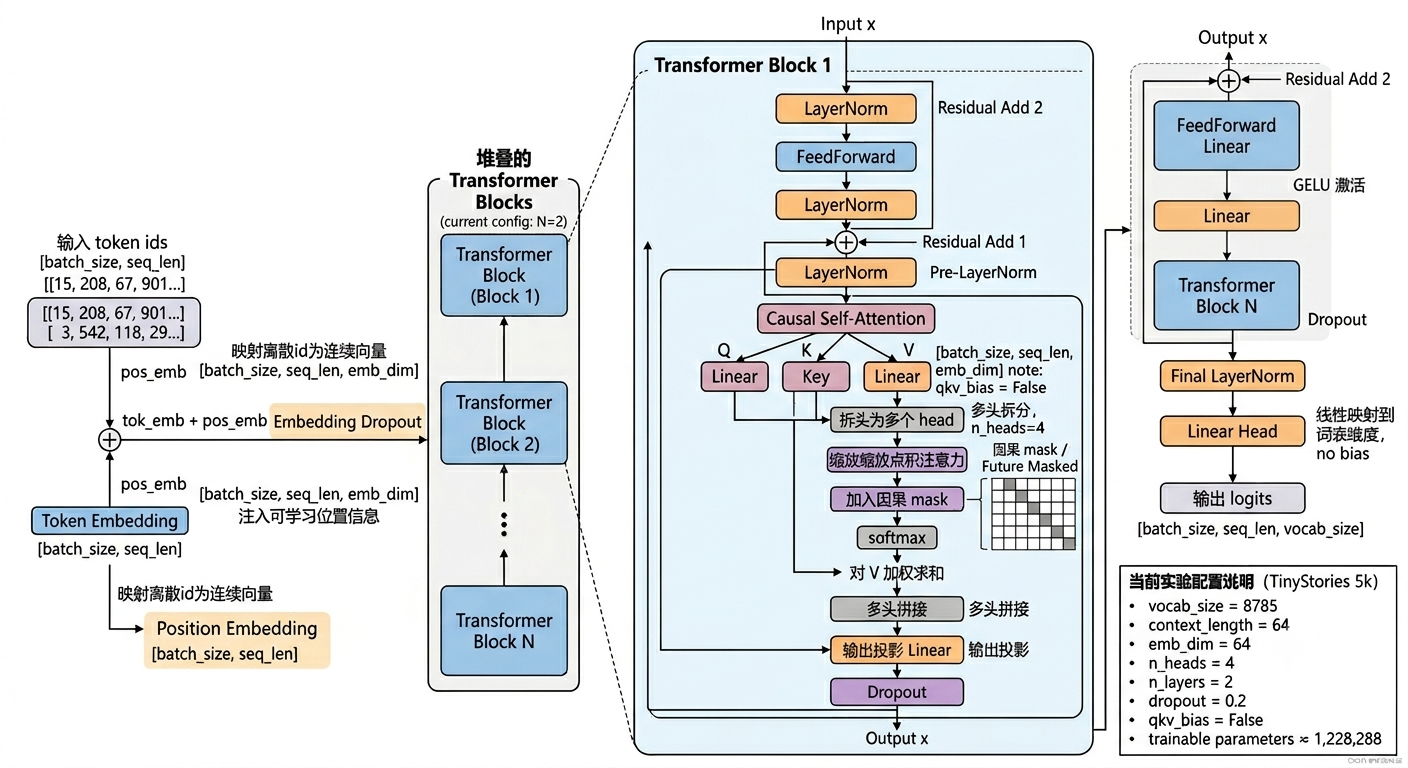
\includegraphics[width=0.96\textwidth,height=7.0cm,keepaspectratio]{pic/minigpt模型结构图.png}
  \caption{MiniGPT 模型总体结构图}
  \label{fig:minigpt_structure}
\end{figure}

图~\ref{fig:minigpt_structure} 体现了小型 GPT 的基本计算路径：离散 token id 首先被映射
为连续向量表示，并与位置编码相加；随后隐藏状态经过多层因果 Transformer 模块建模上下
文关系；最后通过最终 LayerNorm 和线性输出层得到词表维度上的 logits。后续预训练、文本
生成和微调实验均建立在这一模型主体之上。

\subsection{核心模块设计}

\subsubsection{MiniGPTConfig 配置类}

\texttt{MiniGPTConfig} 用于集中管理模型结构参数，包括 \texttt{vocab\_size}、
\texttt{context\_length}、\texttt{emb\_dim}、\texttt{n\_heads}、\texttt{n\_layers}、
\texttt{dropout} 和 \texttt{qkv\_bias} 等。这些参数分别决定词表规模、最大上下文长度、
嵌入维度、注意力头数、Transformer 模块层数、正则化强度以及 Query、Key、Value 线性
映射是否使用偏置。

采用配置类的好处是便于在不同实验中快速调整模型规模。例如，当训练平台算力有限时，可
以减小 \texttt{emb\_dim}、\texttt{n\_layers} 或 \texttt{context\_length} 来降低显存占用和
训练时间；当数据规模扩大时，也可以适当增加模型容量。该设计使模型结构和实验参数之间
保持清晰对应，便于后续预训练实验记录和报告分析。

\subsubsection{因果多头自注意力模块}

\texttt{CausalSelfAttention} 是 MiniGPT 中最能体现 GPT 自回归建模机制的模块。输入隐藏
状态首先分别经过线性层映射为 Query、Key 和 Value，然后将嵌入维度按照注意力头数划分
为多个子空间，在每个头中独立计算缩放点积注意力。多头注意力的结果重新拼接后，再经过
输出投影层得到与输入维度一致的表示。

为了保证模型只能根据历史信息预测下一个 token，代码中构造了上三角因果 mask，用于屏蔽
当前位置之后的未来 token。该 mask 通过 \texttt{register\_buffer} 注册为 buffer，因此会随
模型一起移动到 CPU 或 GPU，但不会作为可训练参数更新。随后，程序按照第二章
式~\ref{eq:causal_attention} 所示的缩放点积注意力计算注意力分数，经过 softmax 得到注
意力权重后，对 Value 进行加权求和。最后，多个注意力头的结果被重新拼接，并经过输出投
影得到注意力子层输出。通过该机制，模型在训练时无法利用未来 token，从而与
next-token prediction 的任务目标保持一致。

\subsubsection{前馈网络与 Transformer 模块}

\texttt{FeedForward} 模块对应前馈网络（feed-forward network），采用“两层线性层 + GELU + Dropout”的结构。第一层线性层将隐
藏维度从 \texttt{emb\_dim} 扩展到 \texttt{4 * emb\_dim}，经过 GELU 非线性激活后，再由第
二层线性层映射回 \texttt{emb\_dim}。这种先升维再降维的设计是 GPT 类 Transformer 模块
中的常见结构，用于增强每个位置隐藏表示的非线性表达能力。

\texttt{TransformerBlock} 由因果自注意力子层和前馈网络子层组成，并采用预层归一化（Pre-LayerNorm）
形式。具体来说，每个子层之前先进行 LayerNorm，然后通过对应模块计算输出，最后与原输
入进行残差相加。残差连接有助于信息和梯度跨层传播，LayerNorm 能够稳定训练过程，
Dropout 则用于降低小数据训练时的过拟合风险。通过堆叠多个 \texttt{TransformerBlock}，
MiniGPT 能够逐层建立 token 之间的上下文依赖关系。

\subsubsection{MiniGPT 模型主体}

\texttt{MiniGPT} 是整个模型的主体类，内部定义了词嵌入、位置嵌入、
嵌入 Dropout、多个 \texttt{TransformerBlock}、最终 LayerNorm 和无偏置线性输出层。
在 forward 过程中，模型首先检查输入序列长度是否超过 \texttt{context\_length}；随后根据
当前序列长度自动生成位置编号，并分别计算词嵌入和位置嵌入。
二者相加后经过 Dropout，再依次输入 Transformer 模块、最终 LayerNorm 和线性输出层。

最终得到的 logits 可直接用于预训练阶段的交叉熵损失计算。推理生成时，程序则取最后一个
位置的 logits，根据贪心策略或采样策略选择下一个 token，并将其追加到上下文中继续生成。
因此，\texttt{MiniGPT} 模型主体同时服务于预训练、文本生成和后续微调实验。

\subsection{模型参数配置与低算力适配}

本项目并不追求训练真实大规模语言模型，而是构建一个能够体现 GPT 核心机制的小参数量
MiniGPT。为了适应单机低算力平台，实验中通过较小的 \texttt{emb\_dim}、\texttt{n\_heads}、
\texttt{n\_layers}、\texttt{context\_length} 和 batch size 控制训练成本。同时，
\texttt{qkv\_bias} 默认为 \texttt{False}，输出层采用无偏置线性层，也有助于减少参数量。
Dropout 被用于降低小数据训练中的过拟合风险。

\begin{table}[!htbp]
  \centering
  \caption{小型 GPT 模型主要参数配置}
  \label{tab:minigpt_config}
  \renewcommand{\arraystretch}{1.2}
  \begin{tabular}{lll}
    \toprule
    参数名称 & 含义 & 设置值 \\
    \midrule
    \texttt{vocab\_size} & 词表大小 & $8785$ \\
    \texttt{context\_length} & 最大上下文长度 & $64$ \\
    \texttt{emb\_dim} & 词嵌入维度 & $64$ \\
    \texttt{n\_heads} & 注意力头数 & $4$ \\
    \texttt{n\_layers} & Transformer 模块层数 & $2$ \\
    \texttt{dropout} & Dropout 比例 & $0.2$ \\
    \texttt{qkv\_bias} & QKV 映射是否使用偏置 & \texttt{False} \\
    参数量 & 可训练参数量 & $1,228,288$ \\
    \bottomrule
  \end{tabular}
\end{table}

表~\ref{tab:minigpt_config} 中的参数来自 TinyStories 5k 预训练实验记录。可以看出，模型
通过降低嵌入维度和 Transformer 层数，将可训练参数量控制在约一百二十万级别。相比真实
大语言模型，该规模非常小，但已经足以展示 GPT 类模型中的词嵌入、位置嵌入、
因果多头自注意力、前馈网络、残差连接和 LayerNorm 等关键机制。

代码中还提供了 \texttt{count\_parameters()} 函数，用于统计模型可训练参数量，方便将不同
实验配置下的模型规模写入日志和报告。\texttt{simple\_test()} 则使用随机 token ids 测试模
型输入输出形状，确认输入 $[\mathrm{batch\_size},\mathrm{seq\_len}]$ 后能够得到
$[\mathrm{batch\_size},\mathrm{seq\_len},\mathrm{vocab\_size}]$ 的 logits，从而验证模型结构
搭建正确。

从训练角度看，MiniGPT 前向传播输出的 logits 可直接与右移一位的目标 token 序列计算交叉
熵损失，用于预训练阶段的参数更新；从推理角度看，模型可以根据当前序列最后一个位置的
logits 选择下一个 token，并将其追加到上下文中继续生成。因此，该模型结构同时支持预训练
阶段的 next-token prediction 训练和推理阶段的自回归文本生成。由于模型层数、嵌入维度和
上下文长度均控制在较小规模，模型能够在普通单机环境下完成训练和推理验证。

综上，本章完成了小型 GPT 模型架构的搭建。该模型保留了词嵌入、位置嵌入、
因果多头自注意力、前馈网络、残差连接和 LayerNorm 等核心机制，同时通过较
小参数规模适配单机低算力环境。该部分直接对应课程作业中“小参数量 GPT 类大语言模型架
构搭建”的要求，并为后续预训练、推理生成和微调实验提供模型基础。

\section{训练数据准备与模型预训练实验}

\subsection{TinyStories 数据集与文本预处理}

\textbf{数据集划分。} 本实验采用 Hugging Face 上的 TinyStories 数据集作为预训练语料。
该数据集由大量简短英文故事组成，语言结构相对简单，包含常见人物、动作、对话和基础叙
事关系，适合小参数量 GPT 模型学习基本英文故事生成模式。实验中选取训练集切片
\texttt{train[:5000]} 和验证集切片 \texttt{validation[:500]}，并读取每条样本中的
\texttt{text} 字段作为原始语料。这里的 \texttt{text} 是数据集中存放故事正文的字段名，表示
一条样本的原始文本内容，并不涉及字符级、词级或子词级分词；真正的文本切分工作由后续
分词器完成。

相比单篇长文本，TinyStories 提供了大量相对独立、语言简单的短故事，能够在较小数据规模
下提供更多情节和句式变化，更适合小参数量模型在低算力条件下学习基础英文叙事模式。单
篇长文本虽然也可以用于预训练，但内容风格和上下文更单一，小模型容易学习到局部文本模
式。多个短故事拼接后仍然能形成连续训练序列，同时保留故事样本的多样性，因此更符合本
实验的目标。

\textbf{文本拼接与清洗。} 程序读取每条故事文本后，将多条故事拼接为连续语料，并在不同
故事之间加入故事结束标记，用于区分相邻故事的边界。该标记在代码中表示为
\texttt{<|endoftext|>}，它并不是普通英文单词，而是用于提示模型当前故事已经结束、下一段
文本属于新的故事。这样做不是为了把多个故事当成同一段真实连续情节，而是为了形成可训
练的 token 序列，同时避免模型把两个独立故事误认为同一段连续内容。正则分词器将故事结
束标记作为完整特殊 token 处理，有助于模型识别不同故事之间的边界。文本清洗主要包括统
一 Windows 和 Linux 换行、去除行尾多余空格、压缩连续空行等基础操作。

\begin{table}[!htbp]
  \centering
  \caption{TinyStories 预训练数据统计}
  \label{tab:pretrain_data_stats}
  \renewcommand{\arraystretch}{1.2}
  \begin{tabular}{lll}
    \toprule
    项目 & 训练集 & 验证集 \\
    \midrule
    数据切片 & \texttt{train[:5000]} & \texttt{validation[:500]} \\
    文本字符数 & $4246757$ & $412120$ \\
    token 数量 & $1014146$ & $98828$ \\
    样本数量 & $15846$ & $1544$ \\
    \bottomrule
  \end{tabular}
\end{table}

表~\ref{tab:pretrain_data_stats} 给出了预训练语料的主要统计信息。可以看出，经过分词和
滑动窗口处理后，训练集和验证集均能提供足够数量的 next-token prediction 样本，用于观察
小型 GPT 模型的训练过程和验证集表现。

\subsection{分词编码与训练样本构造}

\textbf{分词器选择。} 本项目的 \texttt{tiny\_tokenizer.py} 中保留了两种分词器实现：
\texttt{GPT2Tokenizer} 和 \texttt{SimpleRegexTokenizer}。前者对应 GPT-2 BPE 子词分词方案，
后者对应本文主实验采用的正则分词方案。两种方案的主要差异如表~\ref{tab:tokenizer_compare}
所示。

\begin{table}[!htbp]
  \centering
  \caption{两种分词器方案对比}
  \label{tab:tokenizer_compare}
  \renewcommand{\arraystretch}{1.2}
  \small
  \begin{tabular}{L{3.0cm}L{5.0cm}L{5.0cm}}
    \toprule
    对比项 & GPT-2 BPE 分词器 & 正则分词器 \\
    \midrule
    代码实现 & \texttt{GPT2Tokenizer} & \texttt{SimpleRegexTokenizer} \\
    分词方式 & 基于 GPT-2 BPE 子词编码 & 按英文单词、数字、标点、换行和特殊标记切分 \\
    词表来源 & 使用 GPT-2 固定词表 & 根据训练语料构建词表 \\
    词表规模 & 较大 & 较小 \\
    泛化能力 & 较强，适合更复杂文本 & 依赖训练语料，泛化能力较弱 \\
    计算开销 & 输出层参数更多，训练开销更大 & 输出层较小，更适合低算力训练 \\
    本项目用途 & 作为可选方案保留 & 作为主实验方案使用 \\
    \bottomrule
  \end{tabular}
\end{table}

真实 GPT 系列模型通常更倾向于使用 BPE 或类似的子词分词方法，这类方法具有更好的开放
词表能力和文本泛化能力。但本文的目标不是训练真实大规模模型，而是在低算力条件下实现
小参数量 MiniGPT。若直接使用 GPT-2 BPE 分词器，会引入较大的固定词表，使词嵌入层和输
出层参数量明显增加。相比之下，正则分词器能够保留较完整的英文单词，并根据 TinyStories
训练语料构建词表，词表规模更小，更适合 CPU 单机训练和课程实验展示。因此，本文最终选
择 \texttt{SimpleRegexTokenizer} 作为主实验方案，同时保留 \texttt{GPT2Tokenizer} 作为可选
实现。本次预训练中，正则分词器由训练语料构建词表，最终词表大小为 $8785$。

\textbf{滑动窗口样本构造。} 文本被编码为 token id 序列后，程序使用滑动窗口构造语言模
型训练样本。每个输入样本为长度 \texttt{context\_length} 的连续 token 序列，目标序列为
输入整体右移一位后的 token 序列，即模型在每个位置都学习预测下一个 token：
\begin{equation}
  \mathbf{x}=(x_1,x_2,\cdots,x_T),\quad
  \mathbf{y}=(x_2,x_3,\cdots,x_{T+1}) .
  \label{eq:pretrain_next_token_sample}
\end{equation}
本实验设置 \texttt{context\_length=64}、\texttt{stride=64}。这种设置不会让相邻窗口重叠，
可以减少训练样本数量和训练时间，同时仍能覆盖 TinyStories 中的主要文本片段。

\subsection{预训练策略与程序实现}

预训练任务采用 next-token prediction。MiniGPT 对每个 batch 输出 logits，程序将 logits 与
右移一位后的目标 token 序列计算交叉熵损失，从而同时优化序列中所有位置的下一个 token
预测误差。优化器采用 AdamW，并设置 weight decay 以提供一定正则化效果。

在程序实现中，预训练样本由自定义数据集类进行封装。分词后的长 token id 序列按照固定上
下文长度和步长切分为多个样本，每个样本由输入序列和右移一位的目标序列组成。随后，
\texttt{DataLoader} 将若干样本组成 batch 送入模型。对于每个 batch，模型输出形状为
$[\mathrm{batch\_size},\mathrm{seq\_len},\mathrm{vocab\_size}]$ 的 logits，再与目标 token
序列计算交叉熵损失。这一过程对应第二章所述的“输入序列—目标序列—批量训练”的
next-token prediction 预训练机制。

在输入模型之前，每个 batch 中的 token id 首先经过 MiniGPT 的词嵌入层转换为连续向量，
同时根据序列位置生成位置编号并加入位置嵌入。词嵌入用于提供 token 内容信息，位置嵌入
用于提供序列顺序信息，二者相加后作为 Transformer 模块的初始输入表示。随后，模型经过
多层因果 Transformer 模块，输出词表维度的 logits，用于计算 next-token prediction 损失。
这样，预训练程序完整包含了“文本分词—token id 编码—词嵌入与位置编码—Transformer 建
模—loss 计算”的流程。

训练过程中，程序定期在训练集和验证集上评估 loss 与 perplexity。Perplexity 由 loss 的指
数变换得到，可以理解为模型预测下一个 token 时的平均不确定性。训练脚本保存验证集 loss
最低时的 best checkpoint，同时保存最后一轮模型，并记录训练参数、metrics、loss 曲线、训
练日志和文本生成样例。实验中设置 early stopping patience 为 $10$，本次主实验按预设的
$20$ 个 epoch 完成。整个预训练过程在 CPU 单机环境下运行，用于验证小型模型在较低算力
平台上的可运行性。

\begin{table}[!htbp]
  \centering
  \caption{MiniGPT 预训练参数设置}
  \label{tab:pretrain_settings}
  \renewcommand{\arraystretch}{1.2}
  \begin{tabular}{ll}
    \toprule
    参数 & 设置 \\
    \midrule
    数据集 & TinyStories \\
    分词器 & 正则分词器 \\
    \texttt{vocab\_size} & $8785$ \\
    \texttt{context\_length} & $64$ \\
    \texttt{stride} & $64$ \\
    \texttt{emb\_dim} & $64$ \\
    \texttt{n\_heads} & $4$ \\
    \texttt{n\_layers} & $2$ \\
    \texttt{dropout} & $0.2$ \\
    batch size & $16$ \\
    epochs & $20$ \\
    learning rate & $3\times10^{-4}$ \\
    weight decay & $0.05$ \\
    训练设备 & CPU \\
    参数量 & $1228288$ \\
    \bottomrule
  \end{tabular}
\end{table}

表~\ref{tab:pretrain_settings} 汇总了本次预训练的主要参数。整体配置延续了小参数量模型
设计思路，通过较小的嵌入维度、层数和上下文长度控制训练成本，同时保留 GPT 类模型的核
心训练流程。

\subsection{预训练结果与生成效果分析}

\textbf{Loss 与 perplexity 变化。} 预训练过程中，训练 loss 和验证 loss 均明显下降。第一
次评估时，验证 loss 为 $7.9660$，对应验证 perplexity 为 $2881.37$；训练结束时，最优验
证 loss 降至 $3.3125$，对应 perplexity 约为 $27.45$。这说明模型对下一个 token 的预测不
确定性显著降低，已经从 TinyStories 语料中学习到一定的英文短故事语言模式。

\begin{figure}[!htbp]
  \centering
  
\includegraphics[width=0.82\textwidth]{pic/pretrain_loss.png}
  \caption{MiniGPT 在 TinyStories 数据集上的预训练 loss 曲线}
  \label{fig:pretrain_loss_curve}
\end{figure}

图~\ref{fig:pretrain_loss_curve} 展示了预训练过程中的 loss 曲线。可以看到，训练初期 loss
下降较快，随后下降速度逐渐减慢；验证 loss 与训练 loss 保持相近趋势，说明模型训练过程
整体较稳定。由于模型规模较小，后期生成质量仍然有限，但 loss 曲线已经能够证明预训练流
程有效运行。

\begin{table}[!htbp]
  \centering
  \caption{预训练主要结果}
  \label{tab:pretrain_results}
  \renewcommand{\arraystretch}{1.2}
  \begin{tabular}{ll}
    \toprule
    指标 & 数值 \\
    \midrule
    初始验证 loss & $7.9660$ \\
    初始验证 perplexity & $2881.37$ \\
    最优验证 loss & $3.3125$ \\
    最优验证 perplexity & 约 $27.45$ \\
    最优 epoch & $20$ \\
    最优 step & $19700$ \\
    最终训练 loss & $3.2659$ \\
    最终验证 loss & $3.3147$ \\
    训练耗时 & 约 $2491\ \mathrm{s}$ \\
    \bottomrule
  \end{tabular}
\end{table}

表~\ref{tab:pretrain_results} 给出了本次预训练的主要结果。最优验证 loss 出现在第 $20$ 个
epoch、第 $19700$ 个 step，最终训练 loss 和最终验证 loss 相差较小，说明模型虽然容量有限，
但在该数据规模下没有出现特别严重的训练集与验证集分离现象。

\textbf{生成样例与效果分析。} 预训练完成后，使用提示词 \texttt{Once upon a time} 进行自
回归生成。生成测试阶段，模型每次根据当前上下文得到最后一个位置的 logits，并据此选择
下一个 token，再将新 token 拼接回输入序列继续生成。程序支持贪心选择和采样生成两类方
式；在采样生成中，可以通过 temperature 调整概率分布的平滑程度，并通过 top-k 限制候选
token 范围。为减少小模型生成时常见的重复现象，程序中还保留了 repetition penalty 和
no-repeat n-gram 等约束策略。本文生成样例主要用于直观观察预训练模型是否学到基本语言
模式，不将其作为唯一评价依据。下面截取一段生成样例：
\begin{quote}
\small
Prompt: Once upon a time

Generated: Once upon a time, there was a little girl named Lily. She decided to her mom and sing for hours. One day, she went to the kitchen and asked her room to the man and she asked Lily got on her mommy and said,"What is so we can be your knee. You have to wait to know what I try my job you do. You can learn you fix you like to play with your parents. Now you will take another things. I wish I do you want to pick for help me."
They look at least and Ben were happy. They looked for his lesson that they had lots of fun!
\end{quote}

从样例可以看出，模型已经能够形成较明显的故事开头和儿童故事风格，生成内容中出现人物、
动作和简单对话，整体形式接近 TinyStories 的短故事叙述。然而，生成文本仍存在语法不稳
定、角色关系混乱、长程一致性不足等问题，例如部分句子中动作搭配不自然，情节推进也不
够连贯。这与模型规模较小、训练数据切片有限以及训练轮次有限有关。总体而言，本实验的
目标不是达到真实大语言模型的生成质量，而是验证小型 GPT 预训练流程能够完整运行，并能
展示出初步的语言建模效果。

本章完成了预训练部分的主要工作，包括 TinyStories 数据准备、文本拼接与清洗、分词编码、
滑动窗口训练样本构造、预训练程序实现、模型预训练以及预训练效果测试与展示。这些内容
对应了课程作业中“完成大模型预训练”的要求，并为后续微调实验提供了预训练模型基础。

\section{微调实验与任务适应}

\subsection{微调任务与监督数据构建}

预训练阶段的 MiniGPT 主要学习根据上下文预测下一个 token，这一目标能够让模型掌握一定的英语短故事语言模式，但尚不能直接完成明确的下游分类任务。为了考察预训练模型的任务适应能力，本文在预训练 MiniGPT 的基础上构建故事结局倾向二分类任务（story ending polarity classification），要求模型根据输入的故事结尾片段判断其结局倾向。

该任务的输入是一段 TinyStories 风格的英文故事结尾文本，输出类别为 \texttt{positive} 或 \texttt{negative}。其中，\texttt{positive} 表示故事结局积极，例如问题得到解决、人物获得帮助、冲突缓和、人物最终安全或开心；\texttt{negative} 表示故事结局消极，例如问题没有解决、人物受伤、失败、伤心、害怕、孤单，或坏结果持续存在。与普通影评或商品评论情感分类相比，该任务与预训练语料的儿童短故事风格更加一致，因此更适合用来展示本项目中小型 GPT 模型的任务迁移过程。

监督数据由 TinyStories 风格文本构建而来。由于原始故事文本不包含分类标签，本文先抽取候选故事结尾，再依据结局倾向进行人工标注。标注时只依据当前文本中呈现的信息判断：如果困难最终被解决，则标为 \texttt{positive}；如果困难没有解决或负面结果仍然存在，则标为 \texttt{negative}；结局不清楚或难以判断的候选样本不进入最终训练集。最终主实验构建了 300 条带标签的故事结尾样本，数据格式由文本字段和标签字段组成。其中，文本字段为故事结尾片段，标签字段为人工标注的结局倾向类别。该格式既便于程序读取，也能够直接对应文本分类任务的输入和输出，具体文件路径见附录。

数据读取后，程序复用预训练阶段保存的分词器对文本进行编码，并根据模型上下文长度进行截断和填充，同时生成 \texttt{attention\_mask}，用于区分真实 token 与填充位置。数据集采用固定随机种子进行分层划分，训练集、验证集和测试集数量分别为 210、45 和 45。由于测试集中正负类别样本数量并非完全相同，除准确率（accuracy）外，本文还报告 precision、recall、F1、macro F1 和 weighted F1，以更全面地衡量模型在不同类别上的表现。表~\ref{tab:finetune_dataset} 给出了微调数据集划分与标签设置。

\begin{table}[H]
  \centering
  \caption{微调数据集划分与标签设置}
  \label{tab:finetune_dataset}
  \begin{tabular}{L{3.2cm}L{3.2cm}L{3.0cm}L{5.0cm}}
    \toprule
    项目 & 设置 & 数量 & 说明 \\
    \midrule
    任务名称 & 故事结局倾向二分类 & 300 & 判断故事结尾为积极或消极 \\
    标签 0 & \texttt{negative} & 120 & 结局消极、问题未解决、人物受伤或难过 \\
    标签 1 & \texttt{positive} & 180 & 结局积极、问题解决、人物安全或获得帮助 \\
    训练集 & train & 210 & 用于参数更新 \\
    验证集 & validation & 45 & 用于选择验证集表现最优的模型 \\
    测试集 & test & 45 & 仅用于最终效果评估 \\
    \bottomrule
  \end{tabular}
\end{table}

\subsection{微调策略与程序设计}

微调模型在预训练 MiniGPT 主体后增加一个线性分类头，而不改变原有 GPT 主体结构。输入文本依次经过词嵌入、位置嵌入、Transformer 模块和最终归一化层后，得到每个 token 的隐藏状态。由于分类任务需要得到整段文本的表示，因此需要对 token 级隐藏状态进行聚合。常见方式包括使用最后一个有效 token 的隐藏状态、对所有有效 token 进行平均池化，或采用最大池化等。最后一个 token 表示更依赖序列末尾信息，对于自回归生成较自然；但故事结局倾向判断往往依赖整段结尾中的多个词句，而不仅是最后一个 token。因此，本文采用平均池化（mean pooling）获得文本级表示，并在池化时排除 padding 位置。该表示随后输入线性分类头，用于输出 \texttt{negative} 和 \texttt{positive} 两个类别的 logits。训练目标使用交叉熵损失。

在初始化方式上，微调程序加载预训练阶段验证集表现最优的 MiniGPT 参数，并复用预训练阶段的分词器和词表，从而保证预训练与微调阶段的 token 编码方式一致。在参数更新策略上，微调程序保留了多种模式：\texttt{head\_only} 只训练新增分类头，适合快速验证分类头是否有效；\texttt{last\_block} 训练最后一个 Transformer 模块和分类头，是训练成本与适配能力之间的折中；\texttt{full} 则使 MiniGPT 主体和分类头全部参与更新，任务适配能力更强，但训练开销和过拟合风险也更高。考虑到本项目模型参数量较小，且微调任务需要充分适配故事结局倾向分类，主实验最终采用 \texttt{full} 全参数微调方案。

从程序流程看，微调阶段首先读取带标签样本，并按照训练集、验证集和测试集进行划分；随后
加载预训练阶段保存的模型参数和词表文件，保证微调阶段的 token 编码方式与预训练阶段一
致；接着构建分类数据集和 \texttt{DataLoader}，将每条文本编码为 input ids、attention mask
和标签。模型前向传播得到类别 logits 后，与真实标签计算交叉熵损失，并通过优化器更新参
数。训练过程中根据验证集表现保存最佳分类模型，最后在测试集上输出预测结果、分类报告
和错误样本。通过这一流程，预训练 MiniGPT 被适配到故事结局倾向二分类任务中。

训练使用 AdamW 优化器，学习率为 $5\times 10^{-5}$，权重衰减为 0.01，batch size 为 8，训练轮数上限为 60。训练过程中根据验证集表现保存最佳模型，并在最终测试时使用该最佳模型，而不是简单使用最后一轮模型。程序记录训练损失、验证损失、accuracy、分类报告、混淆矩阵以及错误样本，用于后续分析模型在不同类别上的表现。表~\ref{tab:finetune_params} 汇总了主实验参数设置。

\begin{table}[H]
  \centering
  \caption{微调实验参数设置}
  \label{tab:finetune_params}
  \begin{tabular}{L{5.0cm}L{8.2cm}}
    \toprule
    参数 & 设置 \\
    \midrule
    微调数据 & 300 条故事结尾标注样本 \\
    初始化方式 & 加载预训练阶段验证集表现最优的 MiniGPT 参数 \\
    分词器 & 复用预训练阶段词表 \\
    参数更新方式 & 全参数微调，MiniGPT 主体与分类头全部参与更新 \\
    文本表示方式 & 平均池化（mean pooling） \\
    最大长度 & 64 tokens \\
    batch size & 8 \\
    learning rate & $5\times 10^{-5}$ \\
    weight decay & 0.01 \\
    epochs & 60 \\
    early stopping patience & 30 \\
    可训练参数量 & 1,228,418 \\
    \bottomrule
  \end{tabular}
\end{table}

\subsection{微调结果与任务效果分析}

最终实验结果由微调程序自动记录，包括训练曲线、测试集预测结果、分类报告和错误样本分析。图~\ref{fig:finetune_loss} 和图~\ref{fig:finetune_acc} 分别展示了微调过程中的 loss 与 accuracy 变化。具体图片文件路径见附录。

\begin{figure}[H]
  \centering
  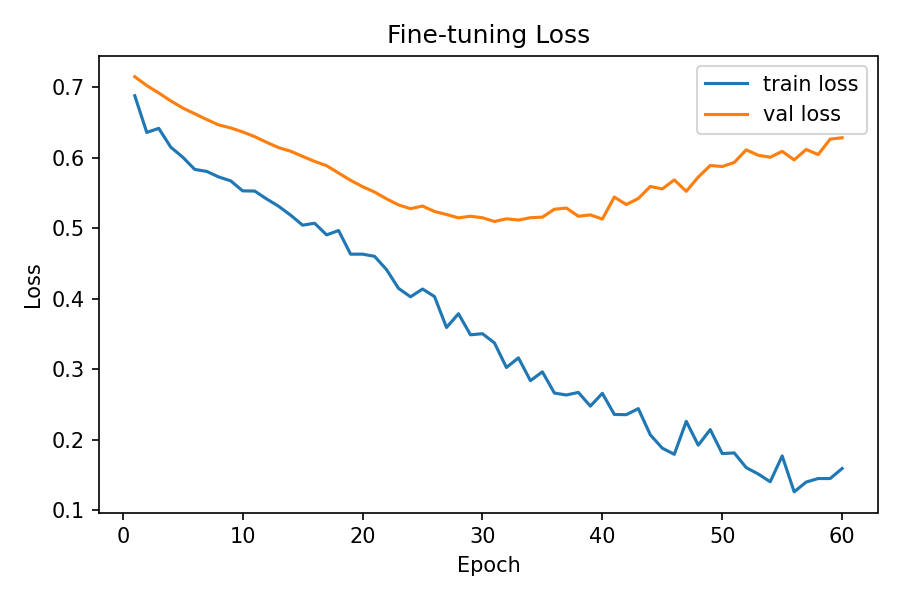
\includegraphics[width=0.86\textwidth]{pic/finetune_loss.png}
  \caption{微调训练 loss 曲线}
  \label{fig:finetune_loss}
\end{figure}

\begin{figure}[H]
  \centering
  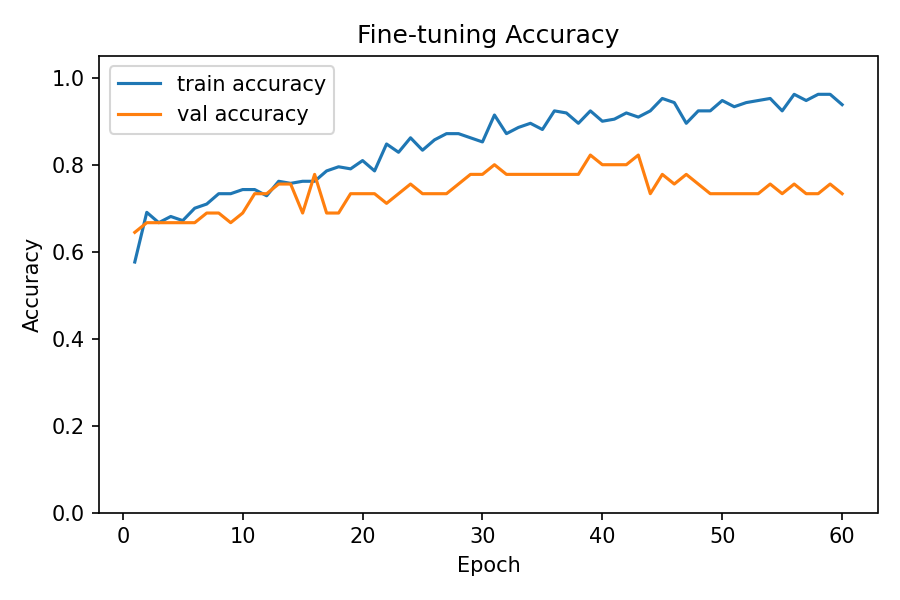
\includegraphics[width=0.86\textwidth]{pic/finetune_accuracy.png}
  \caption{微调 accuracy 曲线}
  \label{fig:finetune_acc}
\end{figure}

从训练过程看，随着 epoch 增加，训练集 loss 整体下降，训练准确率逐步升高，说明模型能够从监督数据中学习故事结局倾向的分类特征。验证集在第 39 轮达到最佳表现，验证准确率为 82.22\%，验证损失为 0.5188。后续训练中，训练集准确率继续升高，而验证集准确率和验证损失出现波动，说明模型后期存在一定过拟合趋势。因此，最终测试阶段使用第 39 轮对应的验证集最优模型进行评估。

在测试集上，模型准确率为 84.44\%，macro F1 为 80.62\%，weighted F1 为 83.87\%。测试集分类指标如表~\ref{tab:finetune_metrics} 所示。混淆矩阵中，真实 negative 被预测为 positive 的样本有 5 条，真实 positive 被预测为 negative 的样本有 2 条，说明模型对 positive 类识别更稳定，而对部分负向结局，尤其是文本中同时包含“学到教训”等积极表达的样本，仍容易发生误判。

\begin{table}[H]
  \centering
  \caption{测试集分类指标}
  \label{tab:finetune_metrics}
  \begin{tabular}{L{3.2cm}L{2.4cm}L{2.4cm}L{2.4cm}L{2.0cm}}
    \toprule
    类别/指标 & Precision & Recall & F1 & Support \\
    \midrule
    negative & 81.82\% & 64.29\% & 72.00\% & 14 \\
    positive & 85.29\% & 93.55\% & 89.23\% & 31 \\
    macro avg & 83.56\% & 78.92\% & 80.62\% & 45 \\
    weighted avg & -- & -- & 83.87\% & 45 \\
    \midrule
    overall accuracy & \multicolumn{4}{l}{84.44\%} \\
    confusion matrix & \multicolumn{4}{l}{tn=9,\ fp=5,\ fn=2,\ tp=29} \\
    \bottomrule
  \end{tabular}
\end{table}

表~\ref{tab:finetune_samples} 给出了部分测试样例及预测结果。可以看到，模型能够较好识别“成为朋友”“安全回家”“得到帮助”等积极结局，也能识别人物受伤、结局悲伤等明显负向结局。错误样例主要集中在边界文本上，例如故事中先出现负面事件，但结尾又包含 “learned to be careful” 一类带有积极含义的表达，模型可能过度关注“学到教训”而忽略前面更关键的负向结果。

\begin{table}[H]
  \centering
  \caption{测试样例与预测结果}
  \label{tab:finetune_samples}
  \begin{tabular}{L{6.2cm}L{1.8cm}L{1.8cm}L{2.4cm}L{2.0cm}}
    \toprule
    文本摘要 & 真实标签 & 预测标签 & 类别概率 & 结果 \\
    \midrule
    Tom and Lucy became good friends. They played and cleaned together every day. & positive & positive & $P_{pos}=0.933$ & 正确 \\
    The pup lay in his hands, still and quiet. The story ends sadly. & negative & negative & $P_{neg}=0.799$ & 正确 \\
    The snake got home safe and sound after being careful in the rain. & positive & positive & $P_{pos}=0.965$ & 正确 \\
    The animals were sad and missed their friend, but learned to be careful. & negative & positive & $P_{pos}=0.905$ & 错误 \\
    The mouse was hurt and could not move, but learned to be careful. & negative & positive & $P_{pos}=0.840$ & 错误 \\
    Timmy and the dog became best friends after going home. & positive & positive & $P_{pos}=0.993$ & 正确 \\
    \bottomrule
  \end{tabular}
\end{table}

与预训练阶段主要用于文本续写不同，微调后的模型能够根据输入故事结尾输出明确的类别标签，说明预训练 MiniGPT 已经能够通过监督数据适配特定分类任务。这一结果表明，即使模型规模较小，只要下游数据与预训练语料在风格上较为一致，预训练模型仍可以通过简单分类头和监督微调获得可观察的任务迁移效果。

\subsection{本章小结}

本章围绕故事结局倾向二分类任务完成了监督微调实验。实验构建了带标签的故事结尾数据，确定了全参数微调与平均池化的分类策略，并在预训练 MiniGPT 基础上实现了分类微调程序。实验通过准确率、F1、混淆矩阵和测试样例展示了模型处理特定任务的效果，测试集准确率达到 84.44\%。同时，结果也表明小模型和小规模数据仍存在局限：模型对 positive 类识别更稳定，对包含负面事件但带有积极措辞的边界样本仍容易误判，后续可通过补充负向样本和改进标注一致性进一步提升泛化能力。

\section{总结与体会}

\textbf{一、成果评价。}

本项目围绕“从零构建大模型”的课程要求，完成了从理论学习到实验实现的完整流程。项目首先梳理了 GPT 类语言模型、分词器、Transformer、预训练与微调等关键知识点；随后基于 PyTorch 搭建了小参数量 MiniGPT 模型，并在 TinyStories 数据集上完成预训练和文本生成测试；最后，通过故事结局倾向二分类任务完成了监督微调实验。整体来看，本项目虽然没有训练真实的大规模商业模型，但在低算力条件下实现了一个可训练、可推理、可微调的小型 GPT 类模型，基本覆盖了课程任务中关于模型搭建、预训练、微调和结果分析的要求。

从实验结果看，预训练阶段模型的 loss 明显下降，生成文本也开始呈现出简单英文故事的结构，说明模型已经学习到一定的语言模式。微调阶段，模型能够根据输入故事结尾判断其倾向类别，说明预训练模型可以通过监督数据适配到特定任务中。这一过程也体现了大语言模型的一般训练思路：预训练主要学习通用语言规律，微调则用于面向具体任务进行适配。

本项目仍存在一些不足，主要原因与模型规模、数据规模和算力条件有关：
\begin{enumerate}
\item 模型参数量较小，生成文本的语法稳定性、情节连贯性和长程一致性仍有限；
  \item 正则分词器泛化能力有限，不如成熟的 BPE 分词器；
\item CPU 训练速度较慢，限制了模型规模、训练轮数和超参数搜索范围；
\item 微调数据规模较小，部分类别边界样本仍容易误判。
\end{enumerate}

后续可以从数据、模型和训练条件三个方面继续改进。首先，可以扩大预训练语料和微调数据规模，使模型接触更多语言模式和边界样本；其次，可以尝试 GPT-2 BPE 等更成熟的分词方案，并适当增加模型层数和隐藏维度；最后，如果具备 GPU 条件，可以进一步增加训练轮数，比较不同模型配置和采样策略对生成效果的影响。

\textbf{二、个人体会与收获。}

通过本次项目，我对大语言模型的底层流程有了更完整的认识。过去使用大模型时，我更多关注的是输入和输出效果，而这次从文本分词、token 编码、词嵌入、位置嵌入，到 Transformer 模块、loss 计算和自回归生成，逐步理解了 GPT 模型内部的基本运行方式。尤其是因果注意力机制让我更清楚地认识到，GPT 的生成过程本质上是在已有上下文条件下不断预测下一个 token。

本次实验也让我更直观地区分了预训练和微调的作用。预训练使模型学习通用语言模式，微调则让模型面向具体任务进行适配。由此也可以理解，不同 AI 工具虽然面向的任务不同，但背后往往都依赖“基础模型能力 + 任务适配”的技术思路。ChatGPT、Codex 以及其他专用 AI 工具并不需要被简单理解为完全不同的技术体系，而可以从模型能力、任务形式和交互方式的差异上进行理解。

此外，这次项目让我更加重视数据处理和训练参数的影响。分词策略会直接决定模型看到的输入形式，语料规模会影响模型能够学习到的语言模式，模型层数、上下文长度、学习率等设置也会影响训练效率和最终效果。在低算力条件下，不能盲目追求更大的模型，而需要在模型规模、数据量、训练时间和实验目标之间取得平衡。

对我个人来说，这次实践也补上了过去模型训练经验中的一部分欠缺。之前在其他任务中使用过模仿学习训练机器人仿真模型，但更多依赖现成代码和 AI 辅助，对底层结构、训练循环和评估指标理解不够。本次虽然训练对象变成了语言模型，但从数据准备、模型搭建、训练调参到结果分析的思路是相通的。通过这次较完整的实践，我对模型训练流程有了更扎实的理解，也相信这些经验能够迁移到今后的其他 AI 项目中。

\section*{参考文献与开源资源说明}
\addcontentsline{toc}{section}{参考文献与开源资源说明}

\begin{enumerate}
  \item Sebastian Raschka, \textit{Build a Large Language Model From Scratch}, Manning, 2024. 本项目在整体学习路线、小型 GPT 模型搭建、预训练和微调流程方面参考了该书的思想。
  \item LLMs-from-scratch GitHub 项目。该开源项目为本文的小型 GPT 架构实现、训练流程设计和实验组织方式提供了参考。
  \item PyTorch 官方文档。本文模型搭建、损失函数、优化器、Dataset 和 DataLoader 等实现参考了 PyTorch 相关说明。
  \item A. Vaswani et al., \textit{Attention Is All You Need}, 2017. 本文关于 Transformer 和注意力机制的理论说明参考了该论文。
  \item Hugging Face Datasets 官方文档。本文使用 TinyStories 数据集时，数据加载、缓存和本地保存流程参考了该文档。
  \item TinyStories 数据集说明。本文预训练语料来源于 TinyStories 数据集，数据集特点和用途参考其公开说明。
  \item tiktoken 分词工具相关资料。本文在分词方案设计中保留 GPT-2 BPE 分词器作为可选方案，相关实现思想参考了 tiktoken 工具说明。
\end{enumerate}

\appendix

\section{项目文件结构}

\begin{verbatim}
my_tiny_gpt/
├── mini_gpt.py
├── tiny_tokenizer.py
├── train_pretrain.py
├── generate.py
├── finetune_classifier.py
├── train_pretrain.ps1
├── data/
│   ├── hf_cache/
│   ├── TinyStories_train/
│   ├── TinyStories_val/
│   └── finetune_300_labeled_detailed.csv
└── outputs/
    ├── pretrain_result/
    └── final_result/

报告/
├── report.tex
└── pic/
\end{verbatim}

\section{主要运行命令}

本项目的主要程序均可在 \texttt{my\_tiny\_gpt/} 目录下运行，具体训练参数已在脚本中统一配置。

\begin{verbatim}
python mini_gpt.py
python tiny_tokenizer.py
.\train_pretrain.ps1
python generate.py
python finetune_classifier.py
\end{verbatim}

\section{主要输出文件}

\textbf{预训练输出。} 预训练实验结果保存在 \texttt{outputs/pretrain\_result/} 中，主要文件包括：
\begin{itemize}
  \item \texttt{vocab.json}：分词器词表与配置；
  \item \texttt{args.json}：预训练运行参数；
  \item \texttt{metrics.json}：预训练关键指标；
  \item \texttt{pretrain\_loss.csv}：训练与验证 loss 记录；
  \item \texttt{pretrain\_loss.png}：预训练 loss 曲线；
  \item \texttt{pretrain\_log.txt}：预训练日志；
  \item \texttt{pretrain\_sample.txt}：预训练模型生成样例；
  \item \texttt{pretrain\_model\_best.pt}：验证集表现最优模型；
  \item \texttt{pretrain\_model\_last.pt}：最后一轮模型。
\end{itemize}

\textbf{微调输出。} 微调实验结果保存在 \texttt{outputs/final\_result/} 中，主要文件包括：
\begin{itemize}
  \item \texttt{args.json}：微调运行参数；
  \item \texttt{metrics.json}：微调关键指标；
  \item \texttt{finetune\_history.csv}：微调训练历史；
  \item \texttt{finetune\_loss.png}：微调 loss 曲线；
  \item \texttt{finetune\_accuracy.png}：微调 accuracy 曲线；
  \item \texttt{classification\_report.txt}：测试集分类报告；
  \item \texttt{finetune\_predictions.csv}：测试集预测结果；
  \item \texttt{finetune\_errors.csv}：错误样本记录；
  \item \texttt{finetune\_classifier\_best.pt}：验证集表现最优分类模型；
  \item \texttt{finetune\_classifier\_last.pt}：最后一轮分类模型；
  \item \texttt{finetune\_sample.txt}：微调模型测试样例。
\end{itemize}

\section{实验结果截图清单}

报告提交或展示时可补充以下截图材料：
\begin{itemize}
  \item 项目目录结构截图；
  \item 分词器测试输出截图；
  \item MiniGPT 模型结构测试输出截图；
  \item 预训练运行过程截图；
  \item 预训练 loss 曲线；
  \item 预训练生成样例；
  \item 微调训练曲线；
  \item 微调分类报告或测试结果截图；
  \item GitHub 仓库文件结构截图。
\end{itemize}

\end{document}
